\documentclass[english, french]{book}
\author{ Gabriel Belouze }

\usepackage{enonce}
\usepackage{tp}
\bcpstUn

\usepackage{amsmath}
\usepackage{amssymb}
\usepackage{amsthm}
\usepackage{array,multicol,multirow} % utility for tables
\usepackage{colortbl}
\usepackage{color}
\usepackage{dsfont}
\usepackage{enumitem}
\usepackage[T1]{fontenc}
\usepackage{graphicx}
\usepackage{ifthen}
\usepackage[utf8]{inputenc}
\usepackage{listings}
\usepackage{mathrsfs}
\usepackage{multicol}
\usepackage{pgf,tikz}
\usepackage{subfig}
\usepackage{upgreek}

\usepackage[outputdir=.build]{minted}
\usemintedstyle{autumn}
\setminted{tabsize=4}

\newtheorem{exercise}{Exercice}[section]
\theoremstyle{definition}
\newtheorem*{remarque}{Remarque}

\newcommand{\myTitle}{ TPs d'informatique en BCPST }
\newcommand{\myName}{ Gabriel Belouze }
\title{\myTitle}
\author{\myName}
\date{}

\excludecomment{correction} % comment this to have corrections


\renewcommand{\chaptername}{TP}

%%  COLORSCHEME
\RequirePackage{xcolor}
\definecolor{halfgray}{gray}{0.55} % chapter numbers will be semi transparent .5 .55 .6 .0
\definecolor{webgreen}{rgb}{0,.5,0}
\definecolor{webbrown}{rgb}{.6,0,0}
\definecolor{Maroon}{cmyk}{0, 0.87, 0.68, 0.32}
\definecolor{RoyalBlue}{cmyk}{1, 0.50, 0, 0}
\definecolor{Black}{cmyk}{0, 0, 0, 0}

%%	HYPERREFERENCES

\PassOptionsToPackage{pdftex,hyperfootnotes=false,pdfpagelabels}{hyperref}
\usepackage{hyperref}  % backref linktocpage pagebackref
\pdfcompresslevel=9
\pdfadjustspacing=1

\hypersetup{
	% Uncomment the line below to remove all links (to references, figures, tables, etc), useful for b/w printouts
	%draft,
	colorlinks=true, linktocpage=true, pdfstartpage=3, pdfstartview=FitV,
	% Uncomment the line below if you want to have black links (e.g. for printing black and white)
	%colorlinks=false, linktocpage=false, pdfborder={0 0 0}, pdfstartpage=3, pdfstartview=FitV,
	breaklinks=true, pdfpagemode=UseNone, pageanchor=true, pdfpagemode=UseOutlines,%
	plainpages=false, bookmarksnumbered, bookmarksopen=true, bookmarksopenlevel=1,%
	hypertexnames=true, pdfhighlight=/O,%nesting=true,%frenchlinks,%
	urlcolor=webbrown, linkcolor=RoyalBlue, citecolor=webgreen, %pagecolor=RoyalBlue,%
	%urlcolor=Black, linkcolor=Black, citecolor=Black, %pagecolor=Black,%
	%------------------------------------------------
	% PDF file meta-information
	pdftitle={\myTitle},
	pdfauthor={\myName},
	pdfsubject={},
	pdfkeywords={},
	pdfcreator={pdfLaTeX},
	pdfproducer={LaTeX with hyperref}
	%------------------------------------------------
}

\newcommand{\subfigureautorefname}{Figure}


% Generate only a singletp
\newboolean{fulltp}
\newcommand{\whenfulltp}[1]{\ifthenelse{\boolean{fulltp}}{#1}{}}
\newcommand{\whennotfulltp}[1]{\ifthenelse{\boolean{fulltp}}{}{#1}}


\newcommand{\tp}{14} % comment me
\whennotfulltp{
    \includeonly{tps/\tp.tex}
    \setcounter{tpCtr}{\tp-1}
}

\begin{document}
\whenfulltp{ \thispagestyle{empty}\maketitle\thispagestyle{empty} }

\whenfulltp{ \part{TPs} }
%! TEX root = ../main.tex

\titre{Boucles \texttt{for} et \texttt{while}}

\commentaire{\NIB{REMARQUES GENERALES :}

	\nipuce toujours commencer par expliquer en français ce que vous allez faire en Python.\\

	\nipuce {\bf Toujours tester sur des exemples !}}

\begin{enonce}

	Il y a deux types de boucles : la boucle FOR et la boucle WHILE.

	La première peut s'utiliser de deux manières :
	\begin{itemize}
		\item soit en explorant les {\bf valeurs} d'un objet {\em itérable} (chaîne de caractères, liste, tuple, range, tableau Numpy) : \texttt{for element in maliste :}
		\item soit en explorant les indices de cet objet : \texttt{for indice in range(len(machaine)) :}
	\end{itemize}

	Dans cet exercice nous voyons différents problèmes où il peut être utile ou nécessaire d'utiliser telle ou telle forme de boucle.\\

	\quessques Que fait la fonction suivante ?

	\begin{verbatim}
def mystere(parametre) :
    x = parametre[0]
    for y in parametre[1:] :
        if y < x :
            x = y
    return x
\end{verbatim}

	\ssques Faire une fonction \texttt{indice\_minimum(maliste)} qui renvoie l'indice de l'élément (ou d'un des éléments) de valeur mnimale dans \texttt{maliste}  (ou suppose sans le vérifier que \texttt{maliste} est formée de nombres).

	\ques Un nombre entier est un {\em palindrome} s'il se lit de la même manière dans les deux sens. Exemples : 2332 ou 56765.

	Un entier $p$ est dit   {\em triangulaire} lorsqu'il existe un entier $n$ tel que $p=1+2+3+\cdots+(n-1)+n$.

	\ssques On veut faire  une fonction \texttt{est\_triangulaire(n)} qui prend un entier $n$ et qui renvoie \texttt{True} si $n$ est triangulaire et \texttt{False} sinon. Complétez-la (y compris les commentaires):

	\begin{verbatim}
def est_triangulaire(n) :
    k = 1 # Cette variable ............
    S = 1 # Cette variable ........
    while ..........
        ...........
        ...........
    return .........
\end{verbatim}


	\ssques Faire une fonction \texttt{est\_palindrome(n)} qui prend un entier $n$ et qui renvoie \texttt{True} si $n$ est un palindrome et \texttt{False} sinon.

	\indic On pourra penser au transtypage \texttt{int --> str}.



	\ssques Faire un script qui donne les 10 premiers entiers qui sont à la fois palindromes et triangulaires.


	\quessques Faire une fonction \texttt{liste\_des\_mots(maphrase)} qui renvoie la liste des mots du \texttt{str} \texttt{maphrase} (deux mots étant séparés par un ou des espaces)

	Exemple : \texttt{liste\_des\_mots('o bladi,      o blada')} doit renvoyer
	\texttt{['o', 'bladi,', 'o', 'blada']}.

	\pagebreak

	\ssques Faire une fonction \texttt{mot\_y\_es\_tu(maphrase,monmot)} qui renvoie \texttt{True} si monmot est un mot de \texttt{maphrase} (séparé du mot précédent et du mot suivant par un ou des espaces, donc) et \texttt{False} sinon.

	\ssques Faire une fonction \texttt{mot\_y\_es\_tu\_II(maphrase,monmot)} qui renvoie la liste (éventuellement vide) des indices des occurrences de \texttt{monmot} dans \texttt{maphrase}.


	\ques Faire une fonction \texttt{dichotomie(f,a,b,epsilon)} qui donne une approximation d'UNE solution de l'équation $f(x) = 0$ sur l'intervalle [a,b] (ou [b,a], peu importe l'ordre). Cette approximation sera donnée à epsilon près.

	Donner un exemple d'application.

	\ques Les {\em diviseurs propres} d'un entier $n$ sont les entiers $k$ tels que $1\leq j< n$ et $k$ divise $n$.

	Les nombres parfaits sont les nombres  égaux à la somme de leurs diviseurs propres. Par exemple $6 =1+2+3.$

	\ssques Faire une fonction \texttt{diviseurs\_propres(n)} qui renvoie la liste des diviseurs propres de $n$, sans doublons.

	On pourra varier les plaisirs en faisant deux versions : l'une  utilisant une boucle \texttt{for} et l'autre une boucle \texttt{while}. Laquelle préférez-vous ?

	\ssques Faire un script qui détermine la liste des 4 premiers \guill{nombres parfaits}.

	\ques En fin de compte, quand utiliser chaque type de boucles ?

\end{enonce}

\begin{correction}


	\commentaire{On va donner deux version : l'une contient une fonction générale de résolution approchée d'équations par dichotomie, qu'on applique à notre problème, et l'autre est directement appliquée au problème.}\\

	\nipuce  \ul{Version 1 contenant une fonction générale} :


	Commençons par  faire une version où l'on fait à part une fonction générale qui donne une approximation d'UNE solution de l'équation f(x) = 0 sur l'intervalle [a,b] (ou [b,a], peu importe l'ordre). Cette approximation sera donnée à epsilon près. Notez comme on peut donner une fonction 'f()' en paramètre. Cette fonction sera définie ailleurs, au moment où l'on a besoin d'appliquer notre fonction dichotomie - voir exemple en commentaire après la fonction dichotomie()

	Pour éviter les erreurs, on va vérifier que f(a) et f(b) sont bien de signes contraires et que epsilon est >0 : on veut éviter qu'une fausse manipulation produise une boucle infinie (epsilon <= 0) ou une solution fausse (si f(a) et f(b) ont même signe). Dans l'un de ces deux cas, on ne renvoie rien et on affiche un message d'erreur.

	\NIB{IMPORTANT} : Notons que si on veut demande d'implémenter l'algorithme de dichotomie au concours, sauf demande explicite, vous n'avez pas besoin de faire cette vérification. Gagnez du temps en indiquant en commentaire "on pourrait commencer par vérifier que... mais ce n'est pas demandé"

	\begin{verbatim}
def dichotomie(f,a,b,epsilon) :

    # On commence par vérifier que f(a) et f(b) sont de signes différents
    # (ou que l'un au moins  est nul)

    # La ligne commentée suivante sert si on veut faire apparaître les étapes de la dichotomie (dans ce cas, il faut la décommenter !).
    # print("a = ",a," et b = ",b, ", et donc |b-a| = ", abs(b-a),".\n On a f(a) = ", f(a), " , f(b) = ", f(b) ," et f(a+b/2) =", f((a+b)/2),"\n" )

    if (f(a)*f(b) <= 0) and (epsilon >0) :
        while abs(b-a) >= 2*epsilon :

            # On va remplacer a ou b par (a+b)/ 2
            # Si f(a) et f(a+b/2) sont strictement de même signe
            # alors notre fonction admet au moins un zéro entre
            # a+b/2 et b, donc on remplace a par a+b/2,
            # sinon c'est b qu'on remplace

            if f((a+b) /2)*f(a) >  0 :
                a = (a+b)/2
            else :
                b = (a+b)/2

            # La ligne commentée suivante sert si on veut faire apparaître les étapes de la dichomie (dans ce cas, il faut la décommenter !).
            # print("a = ",a," et b = ",b, ", et donc |b-a| = ", abs(b-a),".\n On a f(a) = ", f(a), " , f(b) = ", f(b) ," et f(a+b/2) =", f((a+b)/2),"\n" )

        return (a+b)/2
    else :
        print("f(a) et f(b) ont le même signe ou epsilon <= 0")
\end{verbatim}


	\nipuce Avant de passer à l'application à notre problème, voici un exemple simple d'utilisation : On résout l'équation $1-x^2=0$ sur $[0,3]$ à 0.01 près :

	\begin{verbatim}
def fonk(x) :
    return 1-x**2

print(dichotomie(fonk,0,3,0.01)) # on attend 1 à 0.01 près
\end{verbatim}

	\nipuce  Application à l'exercice :
	\begin{verbatim}
from math import cos,pi

def u_n(n,epsilon) :

    def f_n(x) :
        return cos(x) - x/n

    # On définit la fonction f_n() à l'intérieur de la fonction u_n() pour pouvoir utiliser le paramètre n. Sinon on devrait créer uen fonction f_n(n,x) et ça ne collerait pas avec la façon dont est codée la fonction dichotomie (la fonction "f" ne prend qu'un paramètre)

    # On peut bien entendu éviter cette fonction définie dans une fonction en réécrivant la fonction dichotomie spécialement pour ce problème (voir plus bas).

    return dichotomie(f_n, 0, pi/2, epsilon)

# Maintenant on calcule u_n pour une série de valeurs :

N_début= 180
N_fin= 200

eps = 0.0001


for n in range (N_début,N_fin+1) :
    u = u_n(n,eps)
    print ("u_" +str(n),"=",u)
    #print("cosinus :",cos(u), "  x/n :",u/n)
    #print('---')
    print("approximation par le DA à 3 termes",pi/2-pi/(2*n)+pi/(2*n**2))
    print('---------------')
\end{verbatim}



	\nipuce  \ul{Version 2 , écrite spécifiquement pour ce problème} :

	\begin{verbatim}
from math import cos,pi

def f_n(n,x) :
    return cos(x) - x/n

def u_n_v2(n,epsilon) :
    a = 0
    b = pi/2

    while abs(b-a) >= 2*epsilon :

        if f_n(n,(a+b) /2)*f_n(n,a) >  0 :
            a = (a+b)/2

        else :
            b = (a+b)/2

    return (a+b)/2

# Maintenant on calcule u_n pour une série de valeurs :

N_début= 180
N_fin= 200

eps = 0.0001


for n in range (N_début,N_fin+1) :
    u = u_n_v2(n,eps)
    print ("u_" +str(n),"=",u)
    #print("cosinus :",cos(u), "  x/n :",u/n)
    #print('---')
    print("approximation par le DA à 3 termes",pi/2-pi/(2*n)+pi/(2*n**2))
    print('---------------')
\end{verbatim}
\end{correction}

\begin{enonce}
	[Utiliser \texttt{break} ou \texttt{return} pour quitter une boucle]
	Quand on ne sait pas par avance quand la boucle doit s'arrêter, on peut décider de faire une boucle WHILE, mais on a la possibilité, souvent plus simple de faire une boucle FOR qu'on interrompt avec un \texttt{break}. Plus élégamment, dans une fonction, il faut se souvenir que le mot clé \texttt{return} interrompt immédiatement la fonction (et donc la ou les boucles dans lesquelles il se trouve).

	\ques Lire le paragraphe 2.7 du cours de Python.



	\ques Faire une fonction qui prend une liste de nombre en entrée et qui renvoie \texttt{True} s'il y a au moins un zéro parmi eux et False sinon.
	\ssques Avec une boucle \texttt{while}.
	\ssques Avec une boucle \texttt{for} et un break.
	\ssques Avec une boucle \texttt{for} et un ou des return bien placés

	\ques Idem pour  une fonction qui prend une liste de nombres en entrée et qui renvoie \texttt{True} s'ils sont tous nuls et False sinon.




\end{enonce}

\begin{correction}

\end{correction}

%! TEX root = ../main.tex

\titre{Les types python}

\commentaire{D'une manière générale, vous n'avez pas le droit d'utiliser de fonction préprogrammée de Python qui résoudrait directement le problème (comme la fonction \texttt{max()} pour la question \ref{maximum}, par exemple). Il s'agit ici de faire des boucles, des onditions, éventuellement d'utiliser les {\em listes par compréhension} (si vous les maîtrisez). \\

Pour chaque question, commencez par vous demandez quels sont les paramètres de la fonction demandée (et si elle en a !), et ce qu'elle doit renvoyer (et si elle doit renvoyer quelque chose !).\\

A l'écrit, la plupart du temps on vous imposera un nom de fonction, en vous indiquant au passage le nom des paramètres - c'est beaucoup plus simple à corriger, et cela évite des erreurs inutiles pour le candidats, livrés à eux-même devant leur copie. A l'oral vous n'aurez pas forcément cette aide.}


\commentaire{Ce TP vous invite à de nombreuses reprises à consulter le cours de Python. Quand vous tombez sur une telle injonction, si vous maîtrisez déjà le paragraphe demandé, vous pouvez simplement le relire en diagonale pour vérifier et passer à la suite.}

\commentaire{\NIB{Attention !} Vous devez toujours commencer par expliquer en français votre idée avant de l'implémenter. N'oubliez pas de commenter (notamment à quoi servent les variables), utilisez des noms explicites pour vos variables, et mettez des espaces un peu partout pour rendre lisible votre prose (en particulier pour compter les parenthèses\dots)}

\begin{enonce}
[Les booléens]
\ques Que fait la fonction suivante ?

\begin{verbatim}
def mafonc(n) :
    return (n % 2) == 0
\end{verbatim}    

\ques Une fois définie, que produisent les commandes suivante :
\begin{verbatim}
>>> mafonc(3)
>>> mafonc(2)
>>> type(mafonc(3))
\end{verbatim}
\commentaire{Avec-vous compris les mots-clés \texttt{True} et \texttt{False} ? Leur type ? L'intérêt des variables de ce type et le genre d'opérations qu'on peut faire avec ?}

\ques Soit $f : x\lmt \begin{syst}
{rl}
0&\si x\in [0,1]\cup[2,5[\\
1 &\si x\in ]1,2[\\
2&\sinon
\end{syst}$.

Faire une fonction \texttt{foncDeux(x)}, qui prend un réel $x$ et qui renvoie $f(x)$.

\ques Faire une fonction \texttt{foncTrois(x)}, qui prend un réel $x$ et qui renvoie \texttt{True} si $x\in [0,1]\cup[2,5[$ et \texttt{False} sinon.

\ques Que produit la commande suivante :
\begin{verbatim}
>>> True + True + False +True
\end{verbatim}
et celle-ci :
\begin{verbatim}
>>> True * True * False * True
\end{verbatim}


\end{enonce}

\begin{correction}

\end{correction}


\begin{enonce}
[Autour des chaînes de caractères]



\ques Prendre le poly de Python, et vérifier (en faisant les exercices si nécessaire) que vous maîtrisez les paragraphes 4.3.1 et 4.3.2. L'opérateur $+$ est-il commutatif pour les chaînes de caractères ?

\ques Faites un programme qui demande à l'utilisateur :
\begin{itemize}
\item \guill{entrez votre nom} (et qui stocke le nom dans une variable)
\item \guill{{\em{(nom entré précédemment)}, entrez un nombre}} (et qui stocke le nombre dans une variable)
\end{itemize}
et enfin qui affiche :

\cita
{\em (le nom de l'utilisateur)}, le carré de votre nombre est : {\em (suivi de la valeur effective de $x^2$)}
\atic


\ques Prendre le poly de Python, et vérifier (en faisant les exercices si nécessaire) que vous maîtrisez les paragraphes 4.4.1, 4.4.2 et 4.4.3

\ques Faire une fonction \texttt{frequence(machaine, carac)}  qui renvoie la fréquence du caractère \texttt{carac} dans la chaine \texttt{machaine}.

\ques  Faire une fonction  \texttt{remplace\_TOUS\_car(chaine, carac, remplacant)} qui renvoie une copie de la chaine de caract\`{e}res \texttt{chaine} où  toute occurence du  caract\`{e}re \texttt{carac} est remplacée par le caractère \texttt{remplacant}.


\ques  Faire une fonction  \texttt{remplace\_UN\_car(chaine, carac, remplacant)} qui renvoie une copie de la chaine de caract\`{e}res \texttt{chaine} où  la premi\`{e}re occurence du  caract\`{e}re \texttt{carac} est remplacée par le caractère \texttt{remplacant}.



\ques  A l'aide d'une boucle, faire une fonction \texttt{es\_tu\_la(chaine, mot)} qui renvoie \texttt{True} si la chaine \texttt{mot}  est présente dans la chaine de caract\`{e}res \texttt{chaine}.

\commentaire{La commande \texttt{in} permet de faire ça en une ligne (et plus vite). Si vous en avez besoin dans un programme long, vous pouvez l'utiliser, mais dans une question où c'est le BUT comme ici, il faut refaire ça à la main.}

\ques Faire une fonction \texttt{estunpalindrome(machaine)} qui renvoie \texttt{True} si la chaîne \texttt{machaine} est un palindrome et \texttt{False} sinon.

\commentaire{Un palindrome est une chaîne de caractères qui peut être lue dans les deux sens sans changer.}

\ques (après avoir lu le paragraphe 3.9) Même question, mais la différence entre majuscules et minuscules ne doit pas compter.


\begin{enonce}
[A la maison, travail plus long, et nécessitant de savoir lire un fichier texte]

Le but est de pouvoir   déterminer si un texte (de taille suffisante),  donné sous format texte, est en allemand ou en français.
\\

Je ne vous donne pas la structure, seulement des propositions d'étapes,  vous allez devoir  réfléchir  à votre stratégie en amont, et peut-être expérimenter. Lisez donc tout l'énoncé pour vous faire une idée.\\


\nipuce  Trouver sur internet un ou des livre(s) en français en fichier textes (par exemple : \href{http://abu.cnam.fr/} {http://abu.cnam.fr/}).\\

\nipuce  Idem en Allemand.\\

\nipuce Déterminer la fréquence de chaque lettre de l'alphabet dans les corpus précédents.\\

\nipuce Déterminer la fréquence de chaque bigramme (deux lettres qui se suivent) de l'alphabet dans les corpus précédents.\\

\nipuce  Alors ?

\end{enonce}

\begin{correction}

\end{correction}



\end{enonce}

\begin{correction}

\end{correction}


\begin{enonce}
[Autour des listes]

\ques Prendre le poly de Python, et vérifier (en faisant les exercices si nécessaire) que vous maîtrisez les paragraphes 4.5.1 et 4.5.2, puis le paragraphe 3.9.

\ques Considérons le script suivant. 
\begin{verbatim}
import matplotlib.pyplot as plt
from math import  sin exp   # A quoi servent ces deux premières lignes

def fonk(x) :
    return sin(x)*exp(x)

def fonction_mystere_1(a,b,n) :
    '''
    Que fait cette fonction ?
    Que représentent ses paramètres ?
    Que renvoie-t-elle ?
    '''
    reponse = [a]
    p = (b-a)/n # A quoi sert cette variable ?
    for k in range(n+1) :
        reponse.append(a+k*p)
    return reponse

def fonction_mystere_2( l, f) :
    '''
    Que fait cette fonction ?
    Que représentent ses paramètres ?
    Que renvoie-t-elle ?
    '''
    reponse = []
    for element in l :
        reponse.append(f(element))
    return reponse

a , b = -1,  10
# A quoi servent a et b ?  Ce 'a' est-il le même que celui de la fonction_mystere_1() ?

Nb = 1000 # A quoi sert cette variable ?

x = fonction_mystere_1(a,b,Nb)
y = fonction_mystere_2(x, fonk)

plt.figure("ceci n'est pas un graphe") 
plt.plot(x,y)
plt.show()
\end{verbatim}
\ssques Que fait-il ? (en une ligne)
\ssques Répondre aux questions posées en commentaire (ce seraient les commentaires à aire dans le code)

\ssques Pourquoi avoir défini à part la fonction \texttt{fonk(x)} plutôt que la mettre directement où on en a besoin ?
%\ssques A quoi servent  les fonctions \texttt{fonction\_mystere\_1} et \texttt{fonction\_mystere\_2} ?

\ssques (optionnelle ! question à faire après avoir compris le paragraphe 4.5.8 du cours de Python, qui est optionnel au programme)
Redéfinir les deux fonctions précédentes à l'aide de la syntaxe \guill{en compréhension}.

\ques Considérons la suite définie par $u_0=2$ et $\forall n\in\N, u_{n+1}=\sqrt{1+u_n^2}$.

\ssques Faire une fonction \texttt{unTerme(n)} qui renvoie le $n°$ terme de la suite.

\ssques Faire une fonction \texttt{listeDeTermes(n)} qui renvoie la liste $[u_0,u_1,\dots,u_n]$.

\ssques En utilisant le module matplotlib, faire une fonction \texttt{traceTermes(n)} qui trace les termes $[u_0,\dots u_n]$

\ssques Faire un fichier python \texttt{suites\_recurrentes.py} contenant des variantes des fonctions précédentes permettant de faire les opérations considérées en tapant simplement dans le fichier le premier terme $u_0$ et  la fonction de récurrence (\cad la fonction $f$ telle que $u_{n+1}=f(u_n)$).

\ques \label{maximum}Faire une fonction \texttt{maximum(maliste)} qui renvoie le maximum de la  liste \texttt{maliste}, supposée composée de nombres.




\ques  Faire une fonction \texttt{estendouble(maliste, objet)} qui v\'{e}rifie si l'objet \texttt{objet} est pr\'{e}sent (au moins) en double dans la liste \texttt{maliste} (renvoie \texttt{True} dans ce cas, et \texttt{False} sinon.)

\ques  Faire une fonction \texttt{yadesdoubles(maliste)} qui v\'{e}rifie si la liste \texttt{maliste} contient au moins un élément en double (renvoie \texttt{True} dans ce cas, et \texttt{False} sinon.).


%\ques  Faire une fonction qui d\'{e}termine si une liste est un palindrome ou non



%\ques  Faire une fonction d'arguments $L$ et $elt$ qui d\'{e}termine dans la liste d'\'{e}l\'{e}ments $ L$ la position du plus long encha\^{\i}nement de l'\'{e}l\'{e}ment $elt$.

\end{enonce}

\begin{correction}

\end{correction}

\begin{enonce}
[Caractère \guill{en place} (ou pas) d'une fonction prenant une liste en paramètre]

\commentbox{Avant de vous faire travailler, commençons par expliquer le concept d'algorthme \guill{en place}.}


  Un algorithme (cas typique un algorithme de tri de listes) est dit \guill{en place} lorsqu'il ne renvoie pas de résultat, mais modifie  la liste donnée en paramètre.
\\



\nipuce Avant de donner des exemples, il faut bien comprendre que ceci n'a de sens que pour les paramètres de type \texttt{list} ! En effet, c'est le seul type de variable {\em mutable} qui soit au programme en BCPST, et par conséquent, le seul type de variable qu'on puisse modifier au sein d'une fonction. Exemple :


\begin{verbatim}
>>> ma_chaine = "bou"
>>> ma_liste = [6,7,8]
>>> ma_chaine[0] = "Z"

Traceback (most recent call last):
  File "<console>", line 1, in <module>
TypeError: 'str' object does not support item assignment

>>> ma_liste[0] = 1
>>> ma_liste
[1, 7, 8]

\end{verbatim}


\commentaire{
Avant les exemples, profitons-en pour rappeler la différence de syntaxe, expliquée  entre autres dans les paragraphe 3.9, 4.3.4 et 4.5.7 du poly de cours,  entre une {\em méthode} et une fonction {\em fonction} (ces deux termes étant à prendre ici au sens de Python).\\

\nipuce une fonction \texttt{ma\_fonction()} s'applique comme une fonction mathématique.

 Syntaxe : \texttt{ma\_fonction(ses\_parametres)}. Exemple : \texttt{len(ma\_liste)}\\

\nipuce une méthode \texttt{ma\_methode()} EST ATTACHEE à un objet par l'opérateur \guill{.}. 

Syntaxe: \texttt{mon\_objet.ma\_methode(parametres\_de\_la\_methode)}. 

Exemple : \texttt{ma\_liste.append(un\_objet)}
}


\nipuce \NIB{Passons à l'exemple des méthodes de tri fournies par Python} : la méthode \texttt{sort()} et la fonction \texttt{sorted()}.\\




\nipuce  \ul{La méthode \texttt{sort()}} : Elle implémente un algorithme de tri \guill{en place} :
\begin{verbatim}
>>> maliste = [3,4,1,5]

>>> maliste.sort()

>>> maliste
[1, 3, 4, 5]
\end{verbatim}

Comme cet algorithme est \guill{en place}, cette méthode ne \guill{renvoie} rien :
\begin{verbatim}
>>> maliste = [3,4,1,5]

>>> a = maliste.sort()

>>> print(a)
None
\end{verbatim}






\nipuce  Par contre, la fonction \texttt{sorted()} n'est pas \guill{en place} : elle ne modifie pas la liste donnée, mais crée et renvoie une nouvelle liste :
\begin{verbatim}
>>> maliste = [3,4,1,5]
>>> a = sorted(maliste)
>>> a
[1, 3, 4, 5]
>>> maliste
[3, 4, 1, 5]
\end{verbatim}


\commentaire{Je ne parle pas du caractère \guill{en place} comme d'un but à atteindre mais simplement pour une raison pratique : si vous utilisez un algorithme, il faut ben savoir s'il produit une nouvelle liste ou s'il modifie celle qu'on lui donne !}\\

Allez, à vous maintenant :

\ques Avez-vous compris ce qui précède ?

\ques  Lire le paragraphe 4.5.3  et le paragraphe 4.5.6 du cours de Python (en faisant bien par le dernier exercice).




\end{enonce}

\begin{correction}

\end{correction}


\begin{enonce}
[Approfondissons les itérables : chaînes de caractères, listes, mais aussi \guill{tuples} et \guill{range}]

Il serait temps de maîtriser entièrement les paragraphes 4.4 et 4.5 du poly de cours ! 


\end{enonce}


\begin{correction}

\end{correction}

%! TEX root = ../main.tex

\titre{Lecture et écriture d'un fichier texte}

Python permet de lire et d'écrire dans des fichiers (texte, par exemple). Cette fonctionnalité peut être utilisée pour séparer le code en lui-même des données qu'il utilise (par exemple, un fichier de configuration, des données expérimentales, un niveau dans un jeu,etc.) ou qu'il crée (par exemple, un résultat de simulation, une sauvegarde d'un jeu, etc.).

\commentaire  {Avant tout, il est bon de comprendre que Python considère à tout instant que tout fichier que vous voulez manipuler (lire, écrire) est dans ce qu'on appelle le \bi{répertoire courant} ou {\em Current Working Directory (CWD)}. Ce concept peut être vu dans le poly \bi{Annexe I} plus en détails. Ce dossier a une valeur par défaut (que vous n'avez pas forcément choisie !) c'est le dossier dans votre ordinateur où Python va chercher les fichiers que vous voulez lire, et où il va stocker les fichier que vous allez écrire. Il est donc capital de pouvoir choisir ce dossier ! \\

Le programme d'informatique en BCPST précise que vous devez savoir déterminer et changer votre CWD. Voici la procédure, \bi{puis nous verrons comment Pyzo nous évite de recourir à cette syntaxe compliquée} :\\

\nipuce \ul{Pour savoir quel est le répertoire courant} :\\


\texttt{import os }

\texttt{print('Le répertoire courant est :', os.getcwd())}\\



\nipuce \ul{Pour changer le répertoire courant} :

\texttt{os.chdir('''D:/Nouveau\_Repertoire\_Courant/''')}
\\

\nipuce \bi{Mais dans Pyzo on peut éviter ces complications} (qui sont néanmoins au programme, bien que marginales\dots). En effet le menu \texttt{Exécuter} (ou \texttt{Run} contient plusieurs commandes utiles :
\begin{itemize}
	\item \texttt{Exécuter Fichier} (ou \texttt{Execute File}) -- raccourci Ctrl-E (ou Cmd-E sur mac) : exécute tout le fichier.
	\item \texttt{Exécuter Sélection} (ou \texttt{Execute selection}) -- raccourci alt-ENTER : exécute seulement la sélection.
	\item Celle qui nous intéresse ici : \texttt{Exécuter Fichier comme un script} (ou \texttt{Run File as script}) -- raccourci -Maj-Ctrl-E (ou Maj-Cmd-E sur mac) : exécute tout le fichier {\bf MAIS COMMENCE par faire en sorte que le CWD soit choisi comme étant le dossier qui contient le fichier Python exécuté}. \\

	      Ainsi  commencez par créer (et sauvegardez, même s'il n'y a rien dedans) le fichier que vous allez utiliser dans ce TP dans un dossier précis (par exemple nommé \guill{TP3}), et mettez tout  fichier que vous souhaitez lire dans le même dossier. \guill{Exécute ce fichier comme un script}, et désormais votre CWD sera le dossier contenant ce fichier python (donc le dossier nommé {\em TP3} si vous avez suivi\dots)

\end{itemize}
}

\begin{enonce}
	[Premiers pas]

	Tester les instructions suivantes dans un script en s'assurant de comprendre chaque étape.

	\ques	Création de fichier.\\

	Ecrire :
	\begin{verbatim}nom_du_fichier = "fichier_test.txt"\end{verbatim}

	Pour créer un fichier, il faut d'abord l'ouvrir, avec l'option \begin{texttt}"w"\end{texttt}, pour \begin{texttt}"write"\end{texttt} :\\

	\begin{verbatim}ce_fichier = open(nom_du_fichier, 'w')\end{verbatim}


	Pour écrire dans le fichier :

	\begin{verbatim}ligne_1 = 'Fichier écrit un jour froid de février 2013'
ligne_2 = 'La fonction write ne peut prendre que du texte en argument'
ce_fichier.write(ligne_1)
ce_fichier.write(ligne_2)
\end{verbatim}

	On peut aussi y stocker des variables numériques, mais..

	\begin{verbatim}
ligne_4 = 43
ce_fichier.write(ligne_4)
\end{verbatim}


	\dots cette dernière instruction renvoie une erreur : il faut convertir les nombres en texte avant de les écrire dans le fichier.

	\begin{verbatim}
ce_fichier.write(str(ligne_4))
\end{verbatim}

	Ne pas oublier de fermer le fichier une fois qu'on a terminé !
	\\

	\NIB{Conseil :} dès que vous utilisez \begin{texttt}"open"\end{texttt}, écrire l'instruction \begin{texttt}"close"\end{texttt} correspondante. Sinon le fichier restera ouvert en prenant une part de mémoire vive de l'ordinateur et ne pourra pas être modifié par d'autres programmes.

	\begin{verbatim}ce_fichier.close()\end{verbatim}

	Un nouveau fichier a maintenant été créé : le retrouver sur le disque et l'ouvrir (avec le bloc-notes ou pyzo par exemple).  On remarque que ça n'est pas exactement ce qu'on voulait...
	\ques 	Caractère de fin de ligne.\\

	Un caractère spécial est interprété comme une fin de ligne en informatique : \begin{verbatim} \n\end{verbatim} Il sert à indiquer au programme l'endroit exact où on veut passer à la ligne.

	\begin{verbatim}
ce_fichier = open(nom_du_fichier, 'w')
ce_fichier.write(ligne_1 + '\n')
\end{verbatim}


	On peut écrire plusieurs lignes à la fois (et donc passer une liste en argument au lieu d'une chaîne de caractères):


	\begin{verbatim}
ce_fichier.writelines([ligne_2 + "\n", str(ligne_3)+"\n"])
ce_fichier.close()
\end{verbatim}

	\ques 	Paramètre de la fonction open : \texttt{w, a, r}.\\

	Vérifier que l'on a écrasé le fichier précédent. C'est dû à l'argument de la fonction open : "w"  pour "write"). Pour ajouter du contenu au lieu d'écraser le contenu existant : utiliser "a" pour "append".

	\begin{verbatim}
ce_fichier = open(nom_du_fichier, 'a')
ligne_4 = "Voilà une nouvelle ligne\n"
ce_fichier.write(ligne_4)
ce_fichier.close()
\end{verbatim}

	Vérifier que les lignes déjà présentes du fichier n'ont pas été modifiées.
	\pagebreak
	\ques Lecture d'un fichier. \\

	Pour lire le fichier, on utilise la même fonction mais avec un argument différent (l'argument \begin{texttt}'r'\end{texttt}, comme\dots ? ).

	\begin{verbatim}
ce_fichier = open(nom_du_fichier, 'r') 
lu = ce_fichier.readline()
lu2 = ce_fichier.readline()
ce_fichier.close()
print ('La première ligne lue est :', lu)
print ('La deuxième ligne lue est :', lu2)

\end{verbatim}


	\NIB{Astuces :} \begin{enumerate}
		\item On peut aussi utiliser la méthode \begin{texttt}readlines()\end{texttt} pour lire toutes les lignes du fichier d'un coup. Attention cependant, si le fichier est très gros cela peut causer un ralentissement du système puisque python mettra la totalité du contenu du fichier en mémoire vive.
		\item Un autre moyen couramment utilisé pour lire les lignes d'un fichier est :
		      \begin{verbatim}ce_fichier = open(nom_du_fichier)
for line in ce_fichier:
	print(line)
ce_fichier.close()
\end{verbatim}
	\end{enumerate}
\end{enonce}

\begin{correction}

\end{correction}



\begin{enonce}
	[Lecture $++$]

	\ques Créer une fonction \begin{texttt}lire(nom\_fichier)\end{texttt} renvoyant la liste des lignes présentes dans un fichier à partir du nom du fichier pour seul argument. La tester sur notre fichier précédemment utilisé (donc créé par python) et sur un fichier que vous aurez créé à partir du bloc-notes.\\

	\NIB{Bonus :} Ajouter un deuxième argument à la fonction : le nombre de lignes maximum à lire dans le fichier.

	\ques Créer une fonction \begin{texttt}compte\_lettre(nom\_fichier)\end{texttt} qui renvoie le nombre total de \begin{texttt}"e"\end{texttt} dans un fichier.
	\\

	\NIB{Astuce :} les méthodes \begin{texttt}mot.lower()\end{texttt} et \begin{texttt}mot.upper()\end{texttt} modifient la casse d'une chaîne de caractères. Cela peut être utile si on veut prendre en compte les e majuscules.
	\\

	\NIB{Bonus :}  l'idéal est que la lettre à compter (ici, e) soit un argument.

	\ques Ajouter des \begin{texttt}"\#"\end{texttt} au début de certaines lignes de notre fichier texte (en le modifiant directement à l'aide du bloc-notes).

	Créer une fonction \begin{texttt}lire\_non\_commente(nom\_fichier)\end{texttt} qui renvoie sous forme de liste toutes les lignes du fichier ne commençant pas par un \begin{texttt}"\#".\end{texttt}

\end{enonce}

\begin{correction}

\end{correction}

\pagebreak

\begin{enonce}
	[Ecriture]

	\ques Créer une fonction \begin{texttt}ecrire(nom\_fichier, contenu)\end{texttt} où contenu est une liste de chaînes de caractères. Cette fonction écrira chaque \begin{texttt}"ligne"\end{texttt} de \begin{texttt}"contenu"\end{texttt} dans le fichier \begin{texttt}"nom\_fichier"\end{texttt}.

	Tester cette fonction sur la liste \texttt{contenu} de votre choix. Par exemple :\\

	\begin{verbatim}
contenu = ["The grass was greener","The light was brighter", "The taste was sweeter", "..."]

\end{verbatim}

	\NIB{Astuce :} ne pas oublier le caractère de fin de ligne !

	\ques Créer une fonction \begin{texttt}ajoute\_num(nouveau\_fichier, vieux\_fichier)\end{texttt} qui copie le contenu d'un fichier existant dans un nouveau fichier en ajoutant au début de chaque ligne : \begin{texttt}'ligne'\end{texttt} et le numéro de la ligne. \\

	\NIB{Bonus :} ne pas copier les lignes du fichier existant qui commencent par un \begin{texttt}"\#"\end{texttt}.\\

	Exemple du nouveau fichier obtenu :\\

	\begin{verbatim}
ligne 1 : The grass was greener
ligne 2 : The light was brighter
ligne 3 : The taste was sweeter
ligne 4 : ...
\end{verbatim}

\end{enonce}

\begin{correction}

\end{correction}

\begin{enonce}
	[Fichier de configuration]

	\ques Créer un fichier texte \begin{texttt}config.txt\end{texttt} avec le contenu suivant :\\

	\begin{verbatim}# Fichier de configuration pour affichage de polynôme
a = 2
b = 1 
c = 10
bornes = [-10,10]

\end{verbatim}

	\ques Créer un script ou une fonction qui lit ce fichier dans python et crée les variables correspondantes (a, b, c, bornes) en leur affectant les valeurs données dans le fichier.\\

	\NIB {Astuce :} pour trouver l'indice d'un caractère particulier dans une chaîne : \begin{texttt}chaine.find(caractere)\end{texttt}
	pour séparer une chaîne de caractère en une liste de plusieurs éléments séparés par un caractère particulier : \begin{texttt}chaine.split(separateur)\end{texttt}

	\ques Créer une fonction \begin{texttt}voir\_polynome(nom\_fichier)\end{texttt} qui appelle la fonction de l'exercice 7 du TP3 en utilisant les valeurs extraites du fichier comme coefficients du polynôme. On affichera donc la fonction $x \lmt 2x^2 + x -10$.\\

	\NIB{Astuce :} une fonction que l'on a créée nous-même peut être importée comme toute autre fonction en faisant appel au fichier (module) dans lequel elle a été définie : \begin{verbatim}from TP_3_ex_7 import voir_poly\end{verbatim}

	\ques Modifier les valeurs directement dans le fichier texte et vérifier que l'affichage de la fonction (et le calcul des racines) est modifié en conséquence.

\end{enonce}

\begin{correction}

\end{correction}

\pagebreak
\begin{enonce}
	[Stockage de résultat]

	\quessques Comme dans le TP2 (oui, c'est vieux), afficher à l'écran la date et l'heure actuelles.
	Indice : utiliser la fonction \texttt{datetime.now()} du module \texttt{datetime}.

	\ssques Créer une fonction \begin{texttt}save\_time(nom\_fichier)\end{texttt} qui prend en argument un nom de fichier (par exemple, \begin{texttt}"resultat.txt"\end{texttt}) et y écrit une ligne avec la date et l'heure d'exécution de la fonction.
	Si le fichier n'existe pas, il faudra le créer ; dans le cas contraire, on ne veut pas écraser son contenu mais ajouter des nouvelles lignes.
	Tester cette fonction à plusieurs reprises pour créer plusieurs lignes.\\

	\indic la fonction \begin{texttt}os.path.isfile(nom\_fichier)\end{texttt} permet de tester l'existence d'un fichier.

	\quessques Modifier la fonction \begin{texttt}voir\_polynome\end{texttt} de l'exercice 4 pour qu'elle renvoie une liste avec les coordonnées des racines trouvées.

	\ssques Créer une fonction \begin{texttt}sauver\_res(nom\_fichier\_config, nom\_fichier\_res)\end{texttt} qui combine les fonctions \begin{texttt}voir\_polynome()\end{texttt} et \begin{texttt}save\_time()\end{texttt} pour sauvegarder dans un fichier résultat les coordonnées des racines trouvées, à partir du fichier de configuration, ainsi que la date d'exécution de la fonction.



\end{enonce}

\begin{correction}

\end{correction}

%! TEX root = ../main.tex

\titre{Boucles imbriquées}

On a vu précedemment comment faire des itérations simples, avec les boucles \textit{for} et les boucles \textit{while}. On a également rencontré quelques petits exemples de boucles imbriquées : c'est ce qu'on va explorer un peu plus avec ce TP.

\ques Ecrire un programme qui affiche les tables de multiplication de 0 à 10. \\
\NIB{Bonus :} Et si on veut seulement certaines tables de multiplication, comment pourrait-on modifier ce programme ? Ecrire une fonction \texttt{multiplication(liste\_de\_nombres)} qui affiche la table de multiplication de chaque nombre contenu dans la liste \texttt{liste\_de\_nombres}.

\ques \textit{Menu du jour}

Ecrire un programme qui compose un menu du jour pour chaque jour de la semaine, de manière aléatoire : faire une liste d'entrées, une liste de plats, une liste de desserts et tirer, pour chaque jour, une entrée un plat et un dessert. Ce programme affichera les menus sous la forme : "Le menu du \textit{<jour>} est : \textit{<entrée>, <plat>, <dessert>.}"\\

Exemple :
\begin{minted}{python}
entrees = ["salade","soupe à l'oignon","restes de la veille"]
\end{minted}

\NIB{Indication :} vous pourrez importer la fonction \texttt{choice} du module \texttt{random} pour choisir au hasard un élément de chaque liste. Rappel de la syntaxe pour l'importation : \texttt{from random import choice}. Si vous ne savez pas comment utiliser cette fonction, utilisez \texttt{help} !

Il est aussi possible d'importer tout le module \texttt{random} avec \texttt{import random}, auquel cas, la fonction dont on a besoin s'appelera \texttt{random.choice}, et non pas juste \texttt{choice}, ce qui permet d'indiquer d'où vient cette fonction.

\ques \textit{Tableaux en deux dimensions}\\
	Un tableau en deux dimensions peut être vu comme une liste de listes : une liste contenant la liste des lignes, chaque ligne étant représentée par une liste contenant ses coefficients : \[
		T = \begin{bmatrix}
			[ligne 1] \\
			[ligne 2] \\
			[ligne 3] \\
		\end{bmatrix}
	\]
	Pour créer une tel tableau, on peut donc créer une liste de listes, par exemple :

	\begin{minted}{python}
        tablo = [[1, 2, 3], [4, 5, 6], [7, 8, 9]]
    \end{minted}

	qui représente le tableau \[
		\begin{bmatrix}
			1 & 2 & 3 \\
			4 & 5 & 6 \\
			7 & 8 & 9
		\end{bmatrix}
	\]


	Strictement parlant, un tableau en python est de type \texttt{array}, un type d'objet qu'on approfondira plus tard. Ici, je parlerai donc de tableau même lorsque l'objet considéré est de type \texttt{list}. \\
	Si on veut transformer une liste de listes en \texttt{array}, il suffit d'importer le module \texttt{numpy} avec \texttt{import numpy as np}, puis de \textit{transtyper} la liste dont on dispose, c'est-à-dire \textit{changer son type} (comme avec les fonctions \texttt{int} ou \texttt{str} qu'on a déjà rencontrées), en utilisant la fonction \texttt{np.array} :

	\texttt{tableau\_de\_type\_array = np.array(liste\_de\_liste)}

\ssques Créer un tableau \texttt{test} de format 3x3, contenant des variables numériques de votre choix.

\ssques Ecrire une fonction \texttt{montrer\_coef(tableau)} qui affiche tous les coefficients de \texttt{tableau} un par un, en suivant l'ordre de lecture (c'est-à-dire ligne par ligne). \\
Testez cette fonction sur le tableau \texttt{test}.

\ssques Ecrire une fonction \texttt{max\_2D(tableau)} qui prend en entrée un tableau à deux dimensions et renvoie son maximum. \\
Testez cette fonction sur le tableau \texttt{test}.

\quessques Ecrire une fonction \texttt{plus\_proche\_voisin(liste,k)} qui prend en entrée une liste de nombres et un nombre k, et renvoie le coefficient de la liste le plus proche de k.

\ssques Ecrire une fonction \texttt{deux\_valeurs\_plus\_proches(liste)} qui prend en entrée une liste de nombres et renvoie les deux valeurs les plus proches de cette liste.



Le triangle de Pascal est un tableau triangulaire composé comme suit :

- la première ligne, d'indice n=0, est composée d'un seul 1


- pour construire les coefficients de chaque ligne suivante, on additionne le coefficient au-dessus avec celui au-dessus à gauche, en considérant les espaces vides comme des 0. Chaque ligne a donc un coefficient de plus que celle d'avant, et commence et se termine par un 1.

Les premières lignes du triangles sont donc \[
    \begin{matrix}
        1                      \\
        1 & 1                  \\
        1 & 2 & 1              \\
        1 & 3 & 3      & 1     \\
        1 & 4 & 6      & 4 & 1 \\
          &   & \cdots         \\
    \end{matrix}
\]

Ecrire une fonction \texttt{triangle\_pascal(n)} qui prend en entrée un entier n supérieur ou égal à 2 et affiche successivement les lignes du triangle de Pascal jusqu'à la ligne d'indice n. Vous pourrez pour cela utiliser deux listes de nombres, tel que lorsqu'on calcule les coefficients de la ligne \texttt{k}, on ait une liste contenant la ligne \texttt{k-1} et l'autre contenant la ligne \texttt{k}. \\


\NIB{Bonus :} Comment pourrait-on optimiser cette fonction ? \\
Piste : chaque ligne est symétrique.\\


\commentaire{
Il pourra être utile de se souvenir de la méthode de création de liste \textit{par compréhension}, de la forme [\textit{expression} \texttt{for} \textit{element} \texttt{in} \textit{ensemble}], par exemple : \\
\texttt{liste1 = [i**2 for i in range(10)]} ou \texttt{liste2 = [x - 1 for x in liste1]}

Pour ajouter un élément à une liste déjà existante, vous connaissez deux méthodes : \\
- la concaténation :\texttt{liste1 += [10]} \\
- la méthode \texttt{append} : liste1.append(11)
}


\commentaire{\textit{Point culture générale} \\
	Le triangle de Pascal permet notamment de connaître les coefficients du développement de $(a+b)^n$, par exemple pour la ligne \texttt{n=4}:
	\begin{equation*}
		(a+b)^4 = a^4 + 4*a^3b + 6*a^2b^2 + 4*ab^3 + b^4
	\end{equation*}
	Les coefficients de la ligne d'indice 4 du triangle de Pascal sont ainsi :\\
	\texttt{1 4 6 4 1}
}

%! TEX root = ../main.tex

\titre{Matrices}

Quelques manipulations de matrices.

\ques Créer deux matrices 3x3 \verb!test1! et \verb!test2!.

\quessques Ecrire une fonction \verb!somme_matrices(A,B)! qui vérifie si les matrices A et B sont de format compatible, le cas échéant en renvoie la somme A+B, et sinon affiche un message d'erreur. \\

\NIB{Bonus pour les rapides :} et si, plus généralement, on veut faire une combinaison linéaire des matrices A et B, de la forme $a*A + b*B$, avec $a,b \in \mathds{R} $ ?

\ssques Testez votre fonction sur vos deux matrices test.

\quessques Ecrire une fonction \verb!produit_matriciel(A,B)! qui vérifie si les matrices A et B sont de format compatible, le cas échéant en renvoie le produit matriciel A*B, et sinon affiche un message d'erreur.

\ssques Testez votre fonction sur vos deux matrices test. Puis testez-la sur deux autres matrices de formats différents, pour vous assurer du format de la matrice renvoyée.

\quessques Ecrire une fonction \verb!transposee(A)! qui renvoie la transposée de A. \\
\NIB{Rappel (ou découverte) :} la transposée d'une matrice $A_{ij}$ est la matrice $A^T = A_{ji}$, c'est-à-dire qu'on inverse les lignes et les colonnes.

\ssques Testez votre fonction avec les matrices test dont vous disposez.

Manipulation de tableaux avec \verb!numpy!. \\
Commencez par importer \verb!numpy! avec \verb!import numpy as np!. \\

\commentaire{On va découvrir un nouveau type de variable : les arrays. Ce sont des tableaux au sens strict du terme, pas juste des listes de listes. Quel en est l'intérêt ? On peut faire bien plus de calculs avec les arrays, et notamment beaucoup de fonctions existent déjà. Notamment l'équivalent de ce que vous venez de coder.. \\
	On ne vous demandera pas de connaître les différentes et nombreuses fonctions dont dispose \verb!numpy!, mais cela peut être utile d'avoir un aperçu de ce qui existe, notamment pour faire des graphiques facilement plus tard, en TP ou par exemple pour vos TIPE. Retenez que si vous avez besoin de quelque chose pour faire des calcus avec \verb!numpy!, demandez à internet si ça existe et en général la réponse sera oui.}

\ques \textit{Création d'arrays}

\ssques Créez une nouvelle variable \verb!test1_array! en transformant \verb!test1! en array. Pour cela, rien de plus simple, il suffit d'utiliser la fonction \verb!np.array!. \\
\NIB{Rappel :} N'oubliez pas la fonction \verb!help!, qui vous donne accès à la documentation de fonctions !

\ssques Pour créer des tableaux de manière "automatisée", \verb!numpy! dispose de certaines fonctions pratiques. Elles seront particulièrement utile pour faire des graphes. La première qu'on va voir est \verb!np.arange!, qui fonctionne comme \verb!range! : même fonctionnement avec un point de départ, de fin (exclu), un pas. En utilisant cette fonction, créez une liste (array 1D) d'entiers de 1 à 10, une liste des nombres pairs jusqu'à 20 (inclus), et inventez vos propres exemples.

\ssques Une deuxième fonction pratique pour créer des listes est \verb!np.linspace!, qui permet d'avoir des points régulièrement espacés dans un intervalle donné. Regardez ce que renvoie \verb!np.linspace(0,1,10)!, faites d'autres tests.

\newpage
\ques \textit{Manipulation d'arrays}

\ssques Essayez de multiplier \verb!test1! par un entier, puis par un nombre réel non entier. Essayez ensuite avec \verb!test1_array!, que comprenez-vous ?

\ssques De même, essayez d'additionner un scalaire à \verb!test1!, puis à \verb!test1_array!, que comprenez-vous ?

\ssques Que renvoie \verb!test1 + test2! ? et si on fait la même chose, mais avec deux arrays, que se passe-t-il ? Plus pratique que devoir coder une fonction qui fait ça manuellement, non ?

\ssques A l'aide de \verb!np.dot!, faites le produit matriciel de \verb!test1! et \verb!test2!. Attention, cette fonction ne marche qu'avec des arrays. Eh oui, on a codé une fonction qui existait déjà et en mieux.. comme d'habitude finalement !

%! TEX root = ../main.tex

\titre{Introduction à la récursivité}

\commentaire{\textit{Qu'est-ce que la récursivité ?}\\
	Une fonction python peut appeler toute fonction définie (rappelez-vous d'exemples : on a utilisé \verb!abs! par exemple).\\
	En particulier, une fonction peut s'appeler \textit{elle-même} : on dit alors que c'est une \textit{fonction récursive}.
}

Un exemple classique est le calcul de factorielle $n$ : $n!$.
\begin{minted}{python}
def fact(n):
	if (n == 0):
		return 1
	else:
		return n * fact(n-1)
\end{minted}

\exo

\textit{Exponentiation rapide.} Testez à chaque fois vos fonctions !

\ques Ecrire une fonction \verb!puissance_for(x,n)! qui prend en entier un réel \verb!x! et un entier \verb!n!, et renvoie $x^n$, en utilisant une boucle \verb!for! pour calculer le résultat.

\ques Ecrire une fonction \verb!puissance_rec(x,n)! qui fait la même chose, mais en utilisant la récursivité (indice : $x^n = x*x^{n-1}$).

\ques Plus malin, plus rapide !\\
Ecrire une fonction \verb!puissance_rec_rapide(x,n)! qui fait la même chose, en étudiant la parité de \verb!n! pour appliquer des propriétés de la mise en puissance.

\exo

Le format de papier A0 correspond à un rectangle de largeur de 84,1cm et une longueur de 118,9cm. le format A1 est obtenu en coupant en deux parties égales le format A0, il a donc pour longueur la largeur de A0 et pour largeur la moitié de la longueur de A0. Sur le même principe une feuille A1 contient deux feuilles A2, une feuille A2 deux feuilles A3, etc...

Ecrire une fonction récursive \verb!format_papier(n)! prenant en paramètre un entier naturel $n$ et qui retourne longueur et largeur, dans cet ordre, d'une feuille de format An.

\exo

\textit{Suite de Fibonacci}\\
La suite de Fibonacci est définie par :
\begin{equation*}
	u_0 = 0, \\
	u_1 = 1, \\
	\forall n \in \mathds{N}, u_{n+2} = u_{n+1} + u_{n}
\end{equation*}

\ques Ecrire une fonction \verb!fibo(n)! qui renvoie le terme d'indice n de la suite de Fibonacci, de manière itérative (avec une boucle \verb!for!).

\ques Pareil, mais avec la récursivité. Est-ce efficace ? Comment faire mieux ?

%! TEX root = ../main.tex

\titre{Dictionnaires}

%\commentaire{\textit{Un nouveau type de variable : les dictionnaires}\\
Ce sont des structures de données (\texttt{dict}) modifiables et non séquentielles ; un élément n'est pas repéré à l'aide d'un indice mais à l'aide d'un nom (sa \texttt{clef}). Un élément est constitué d'un \texttt{champ} : la donnée d'une clé et d'une valeur.
\begin{enumerate}
	\item La clé est un nombre, une chaîne de caractère (ou un t-uplet, mais ce n'est pas un type de variable qu'on a vu jusque là).
	\item La valeur peut être de type quelconque.
\end{enumerate}
Le nom de dictionnaire ne vient pas de nulle part : cela fonctionne comme un dictionnaire papier, où on range une défintion (un champs) en la repérant grâce à un certain mot (la clef).\\
Le type \texttt{dict} permet la définition de conteneurs dont les valeurs sont repérées non plus par des indices mais par des clés. \\

Visuellement, un dictionnaire est délimité par des acolades : \texttt{\{\}}, et les clefs sont reliées aux champs grâce à deux points : \texttt{:}.\\

Comment définir un dictionnaire ?\\
Un exemple :
\begin{minted}{python}
dict_test = {'clef1':12.5, 'clef2':'deuxieme champs', 3:'champs3'}
\end{minted}
On peut aussi le faire en plusieurs etapes :
\begin{minted}{python}
dict_test2 = {}
dict_test2['clef1'] = 12.5
dict_test2['clef2'] = 'deuxieme champs'
dict_test2[3] = 'champs3'
\end{minted}

On peut ensuite accéder aux champs contenus dans un dictionnaire en appelant les clefs : \mintinline{python}{dict_test['clef1']} renvoie 12.5.
%}

\textit{Entrainement}
\quessques Créez un dictionnaire \texttt{age} contenant les âges de trois personnes différentes, en les repérant par leur prénom, puis un dictionnaire \texttt{taille} contenant leur taille.
\ssques Les valeurs (champs) d'un dictionnaire peuvent aussi être des dictionnaires ! Faites un dictionnaire \texttt{informations} contenant les deux dictionnaires précédents, repérés par une chaîne de caractère chacun.
\ssques Faites un nouveau dictionnaire \texttt{ville\_naissance} contenant, pour les mêmes personnes, leur ville de naissance. Ajoutez ce dictionnaire à \texttt{informations}.

\ques \textit{Opérations sur les dictionnaires}
\ssques Que renvoie la commande suivante ?
\begin{minted}{python}
for x in age :
    print(x)
\end{minted}
Que comprenez-vous sur cette manière de parcourir un dictionnaire ?
\ssques Parcourez chaque dictionnaire contenu dans \texttt{informations} (à l'aide d'une boucle bien sûr), et enlevez une personne des dictionnaires que vous avez faits jusque-là. La fonction \texttt{del} permet d'enlever une clef (et le champ associé) dans un dictionnaire.

\newpage
\ques \textit{Méthodes applicables aux dictionnaires}
Testez les méthodes suivantes sur les dictionnaires dont vous disposez : \\
- \mintinline{python}{D.keys()} (pour un dictionnaire \mintinline{python}{D})\\
- \mintinline{python}{D.values()} \\
- \mintinline{python}{D.items()} \\
- \mintinline{python}{D.copy()} \\
Que comprenez-vous sur ces méthodes, que font-elles ?

\textit{Cryptage de César à l'aide de dictionnaires}
\ques  Définir une variable \mintinline{python}{alphabet = "abcdefghijklmnopqrstuvwxyz"}.
\ques Ecrire un script qui définit un dictionnaire ayant pour clefs les lettre de l'alphabet et pour valeurs leur position dans l'alphabet. Utilisez bien sûr la variable \texttt{alphabet} !
\ques Ecrire une fonction \texttt{cesar(n)} prenant en argument un entier \texttt{n} et qui renvoie un dictionnaire comme en 2, mais dont les valeurs sont décalées de l'entier \texttt{n} modulo 26.
\ques Ecrire une fonction \texttt{cryptage(texte,n)} prenant en argument un texte sous forme d'une chaine de caractère et un entier \texttt{n} et qui le crypte selon le chiffrement de César avec décalage de \texttt{n}.

%! TEX root = ../main.tex

\titre{Algorithmes de tri}


Il existe déjà des fonctions optimisées pour trier des listes. On va les présenter rapidement, comprendre leurs particularités, puis on s'attaquera à en coder nous-mêmes. C'est un très bon exercice d'algorithmique, qui soulève notamment les questions d'optimisation dont on a déjà parlé les fois précédentes. \\

%\commentbox{Avant de vous faire travailler, commençons par expliquer le concept d'algorthme \guill{en place}.}

%  Un algorithme (cas typique un algorithme de tri de listes) est dit \guill{en place} lorsqu'il ne renvoie pas de résultat, mais modifie  la liste donnée en paramètre.

\exo
\textit{Les fonctions et méthodes de tri déjà existantes dans python}\\

\nipuce \ul{La méthode \texttt{sort()}} : Elle implémente un algorithme de tri \guill{en place}\\
\NIB{Algorithme en place ?} Un algorithme (cas typique un algorithme de tri de listes) est dit \guill{en place} lorsqu'il ne renvoie pas de résultat, mais *modifie* la liste donnée en paramètre. \\
\NIB{Méthode ou fonction ?} Une méthode \texttt{ma\_methode()} *est attachée* à un objet par l'opérateur \guill{.}. Par exemple : la méthode \texttt{append} ! Syntaxe : \texttt{mon\_objet.ma\_methode(parametres\_de\_la\_methode)}. \\
Une fonction \texttt{ma\_fonction()} s'applique comme une fonction mathématique. Syntaxe : \texttt{ma\_fonction(ses\_parametres)}.

\begin{Verbatim}[tabsize=4]
	>>> maliste = [3,4,1,5]

	>>> maliste.sort()

	>>> maliste
		[1, 3, 4, 5]
\end{Verbatim}

Comme cet algorithme est \guill{en place}, cette méthode ne \guill{renvoie} rien :
\begin{Verbatim}[tabsize=4]
	>>> maliste = [3,4,1,5]

	>>> a = maliste.sort()

	>>> print(a)
	None
\end{Verbatim}

\nipuce  Par contre, la fonction \texttt{sorted()} n'est pas \guill{en place} : elle ne modifie pas la liste donnée, mais crée et renvoie une nouvelle liste :

\begin{Verbatim}[tabsize=4]
	>>> maliste = [3,4,1,5]
	>>> a = sorted(maliste)
	>>> a
		[1, 3, 4, 5]
	>>> maliste
		[3, 4, 1, 5]
\end{Verbatim}

\ques Faites des tests par vous-mêmes, en faisant attention à si vous créez une nouvelle liste ou modifiez l'existante !

\newpage
\exo
\textit{Tri à bulles}\\
C'est l'algorithme de tri le plus simple :
\begin{enumerate}
	\item [--] Parcourir les éléments du tableau de gauche à droite. \\

	      Dès que l'on rencontre deux éléments consécutifs qui ne sont pas dans le bon ordre, on échange leur position.
	      C'est à dire :\\
	      \texttt{SI tableau[i] > tableau[i+1]}\\
	      \texttt{ALORS : échanger tableau[i] et tableau[i+1]}

	\item[--] Recommencer tant que l'on a changé quelque chose.
\end{enumerate}

Le principe illustré ci-dessus conduit à l'algorithme général suivant pour le tri d'un tableau unidimensionnel (une liste) :
\begin{Verbatim}[tabsize=4]
	Algorithme du Tri à bulle (Paramètre  : un tableau T)
        N = longueur(T)
        Changement = VRAI
        TANT QUE Changement est VRAI :
            Changement = FAUX
            POUR  i variant de 0 à N-2
                SI T[i] > T[i+1]
                ALORS échanger T[i] et T[i+1]
                ALORS Changement = VRAI
            FIN POUR
            N = N-1
        FIN TANT QUE
\end{Verbatim}

\ques Etudiez cet algorithme en pseudo-code. A quoi sert la variable \texttt{Changement} ? Pourquoi i varie entre 0 et N-2 ? Pourquoi N devient N-2 à chaque étape du tant que ? (Ce dernier point est plus délicat : c'est une histoire d'optimisation. Demandez-vous s'il le dernier élément est bien positionné quand on vient de parcourir toute la liste, que faut-il en déduire ?) \\
Cet algorithme est-il en place ?

\quessques Écrire en Python une fonction \texttt{tri\_Bulle(liste)} prenant en paramètre une liste \texttt{liste}, et qui trie \texttt{liste} dans le sens croissant par un tri à bulle.
\NIB{Astuce :} vous pouvez placer des \texttt{print} stratégiques pour visualiser ce que fait l'algorithme étape par étape. Par exemple, regardez quels élément sont déplacés, que devient la liste au fur et à mesure.
\ssques Modifier la fonction pour que le tri se fasse dans l'ordre décroissant.

\exo
\textit{Tri par insertion} \\
Le principe : on constitue (imaginairement) 2 tas : \\
\begin{enumerate}
	\item[--] l'un dans la main droite, contenant toutes les cartes avant tri,
	\item[--] l'autre dans la main gauche, contenant les cartes déjà triées,
\end{enumerate}
Initialement la main gauche est vide. \\

Chaque étape consiste à : \\
\begin{enumerate}
	\item[--] prendre la première carte du tas non trié
	\item[--] L'insérer progressivement à sa bonne place dans le tas trié, en la faisant descendre d'une position tant que sa valeur reste inférieure à celle de la carte située en dessous-d'elle.
\end{enumerate}
Après chaque étape le tas non trié contient une carte de moins, le tas trié une carte de plus.\\
A la fin du tri la main droite est vide. La main gauche contient toutes les cartes, triées. \\

\newpage
En pseudo-code, l'algorithme de Tri par insertion s'écrit :
\begin{Verbatim}[tabsize=4]
	Algorithme de Tri par insertion (Paramètre : un tableau T)
	N = longueur(T)
	# Balayage du tableau du 2ème jusqu'au dernier élément :
	POUR i variant de 1 à N-1:
	x = T[i] 	# C'est l'élément à insérer
	k = i 	# k est son indice
	# Insertion dans la partie triée :
	TANT QUE k > 0 et T[k-1] > x:
	# Décalage d'un cran sur la gauche :
	T[k] = T[k-1]
	k = k-1
	T[k] = x
\end{Verbatim}

\ques Etudiez ce pseudo-code. Comprenez-vous l'étape du décalage vers la gauche ? Pourquoi i varie de 1 à N-1 ?

\ques Ecrire en Python une fonction \texttt{tri\_Insertion(liste)} prenant en paramètre une liste \texttt{liste}, et qui trie \texttt{liste} dans le sens croissant par un tri par insertion.
\NIB{Bonus :} Modifier l'algorithme pour que le tri se fasse dans l'ordre décroissant.

\exo
\textit{Tri par sélection}

Pour un tableau de $N$ éléments, il consiste à :
\begin{enumerate}
	\item[--] Sélectionner la valeur maximale dans le tableau
	\item[--] Le déplacer en dernière position du tableau.
	\item[--] Recommencer avec le tableau des $N-1$ premiers éléments, et ainsi de suite.
\end{enumerate}


\ques Ecrire une fonction \texttt{indiceMax(liste,i)} prenant en paramètre une liste numérique \texttt{T} et un entier \texttt{i} et qui retourne l'indice du plus grand élément de \texttt{liste} d'indice au plus \texttt{i}.
\ques L'utiliser pour écrire une fonction \texttt{tri\_selection()} qui applique l'algorithme de tri par sélection.

\exo
\textit{Tri comptage}

Lorsque on est en présence d'une liste, où la valeur des éléments est connue a priori, et en petit nombre, l'ordonner peut s'exécuter plus rapidement par un tri comptage. Le principe est le suivant :\\
Considérons une liste ne contenant que des 0 et des 1. On la parcourt à l'aide d'une boucle for, pour stocker dans deux variables \texttt{nb0} et \texttt{nb1}, le nombre de 0 et de 1 de la liste. On crée ensuite une nouvelle liste constituée de \texttt{nb0} zéros suivies de \texttt{nb1} uns ; que l'on renvoie.
\ques Ecrire une fonction \texttt{triComptage(L)} prenant en argument une liste \texttt{L} constituée de zéros et de uns,  et qui renvoie la liste ordonnée contenant les mêmes éléments.\\
On pourra l'essayer avec la liste créée de la façon suivante :
\begin{minted}{python}
 from random import randint
 n = 20
 L = []
 for k in range(n):
 	L.append(randint(0,1))
 # ce qui est équivalent à :
 L = [randint(0,1) for k in range(n)]
 # (en utilisant la syntaxe par compréhension)
 \end{minted}

%! TEX root = ../main.tex

\titre{Dichotomie}

Dans ce TP, on s'intéresse à différentes applications de la technique de \emph{dichotomie}. Cette technique est utile pour rechercher un élément dans un espace de recherche (par exemple une liste). Le principe de la recherche dichotomique est de couper l'espace de recherche en deux, successivement jusqu'à trouver l'élément. C'est une technique beaucoup plus efficace que de parcourir l'ensemble des éléments de l'espace, un à un.

\begin{example}
	Dans 'Le Juste Prix', les candidat.es finalistes ont 30 secondes pour deviner à l'euro près la valeur d'une vitrine de cadeaux (et remportent les cadeaux s'iels y arrivent). La vitrine a une valeur maximale de 50.000 euros. Pour ce faire, le/la candidat propose une estimation, et l'animateur lui répond "c'est plus" ou "c'est moins".\\
	La technique optimale consiste à proposer successivement le milieu des bornes du prix. Ainsi:
	\begin{itemize}
		\item On commence par proposer 25.000€
		\item Si c'est plus, on propose 37500€, si c'est moins 12500€
		\item Et on continue comme ça
	\end{itemize}
	Dans le pire des cas, il faudra 16 essais pour trouver le juste prix.
	\commentaire{Pourquoi 16 ? Et si la valeur maximum de la vitrine est 1.000.000€, combien d'essais faudra-t-il au maximum ?}
\end{example}

\begin{enonce} [ Recherche dichotomique dans une liste triée ]
	Dans cet exercice on se pose la question d'écrire un algorithme pour déterminer si un élément appartient à une liste.
	\quessques Écrire une fonction \texttt{find\_naive(l, x)} qui prend en argument une liste \texttt{l1} et un élément \texttt{x} et détermine si \texttt{x} apparaît dans \texttt{L}. La fonction doit renvoyer \texttt{True} ou \texttt{False} en fonction.
	\ssques Tester votre fonction sur quelques exemples.
	\ssques Si \texttt{L} est de taille 10, combien d'éléments est-ce que \texttt{find\_naive} devra regarder dans le pire des cas ? Et si \texttt{L} est de taille 1000 ?

	Dans le cas général, on ne peut pas vraiment faire mieux que de regarder un à un tous les éléments. Mais si \texttt{t} est triée (dans l'ordre croissant), on peut aller beaucoup plus rapidement! En effet si je sais que \texttt{x} est plus grand qu'un élément \texttt{e} de la liste, alors il ne peut pas être à gauche de \texttt{e}. S'il est plus petit, \texttt{x} ne peut pas être à droite de \texttt{e}.

	\begin{example}
		Recherche de \texttt{4} dans le tableau suivant:
		\begin{center}
			\begin{tabular}{cccccccccc}
				\cline{1-9}
				\multicolumn{1}{|>{\centering}p{1.1cm}|}{1} & \multicolumn{1}{|>{\centering}p{1.1cm}|}{2} & \multicolumn{1}{|>{\centering}p{1.1cm}|}{3}
				                                            & \multicolumn{1}{|>{\centering}p{1.1cm}|}{4} & \multicolumn{1}{|>{\centering}p{1.1cm}|}{\cellcolor{Maroon}5} & \multicolumn{1}{|>{\centering}p{1.1cm}|}{6} & \multicolumn{1}{|>{\centering}p{1.1cm}|}{7} & \multicolumn{1}{|>{\centering}p{1.1cm}|}{8} & \multicolumn{1}{|>{\centering}p{1.1cm}|}{9}
				\\
				\cline{1-9}
				\multicolumn{1}{c}
				{\tt{bottom}}
				                                            & \multicolumn{3}{c}{}
				                                            & \multicolumn{1}{c}
				{\tt{mid}}
				                                            & \multicolumn{4}{c}{\null}
				                                            & \multicolumn{1}{c}
				{\tt{top}}                                                                                                                                                                                                                                                                                                                                        \\
				\multicolumn{1}{c}
				{}
				                                            & \multicolumn{3}{c}{}
				                                            & \multicolumn{1}{c}
				{$\mathbf{>e}$}
				                                            & \multicolumn{4}{c}{\null}
				                                            & \multicolumn{1}{c}
				{}                                                                                                                                                                                                                                                                                                                                                \\
				\multicolumn{3}{c}{}
				                                            & \multicolumn{3}{c}{Dichotomie à gauche}     & \multicolumn{4}{c}{}                                                                                                                                                                                                                                  \\
			\end{tabular}
			\begin{tabular}{cccccccccc}
				\cline{1-9}
				\multicolumn{1}{|>{\centering}p{1.1cm}|}{1} & \multicolumn{1}{|>{\centering}p{1.1cm}|}{2} & \multicolumn{1}{|>{\centering}p{1.1cm}|}{\cellcolor{Maroon}3}
				                                            & \multicolumn{1}{|>{\centering}p{1.1cm}|}{4} & \multicolumn{1}{|>{\centering}p{1.1cm}|}{\cellcolor{gray}5}   & \multicolumn{1}{|>{\centering}p{1.1cm}|}{\cellcolor{gray}6} & \multicolumn{1}{|>{\centering}p{1.1cm}|}{\cellcolor{gray}7} & \multicolumn{1}{|>{\centering}p{1.1cm}|}{\cellcolor{gray}8} & \multicolumn{1}{|>{\centering}p{1.1cm}|}{\cellcolor{gray}9} & \multicolumn{1}{c}{\hphantom{top}}
				\\
				\cline{1-9}
				\multicolumn{1}{c}
				{\tt{bottom}}
				                                            & \multicolumn{1}{c}{}
				                                            & \multicolumn{1}{c}{\tt{mid}}
				                                            & \multicolumn{1}{c}
				{}
				                                            & \multicolumn{1}{c}{\tt{top}}
				                                            & \multicolumn{5}{c}
				{}                                                                                                                                                                                                                                                                                                                                                                                                                                                     \\
				\multicolumn{1}{c}
				{}
				                                            & \multicolumn{1}{c}
				{}
				                                            & \multicolumn{1}{c}{$\mathbf{<e}$}
				                                            & \multicolumn{3}{c}{Dichotomie à droite}
				                                            & \multicolumn{4}{c}
				{}
			\end{tabular}
			\begin{tabular}{cccccccccc}
				%\multicolumn{9}{c}{Dichotomie à droite}\\
				\cline{1-9}
                \multicolumn{1}{|>{\centering}p{1.1cm}|}{\cellcolor{gray}1} & \multicolumn{1}{|>{\centering}p{1.1cm}|}{\cellcolor{gray}2}   & \multicolumn{1}{|>{\centering}p{1.1cm}|}{\cellcolor{gray}3}
				                                                            & \multicolumn{1}{|>{\centering}p{1.1cm}|}{\cellcolor{Maroon}4} & \multicolumn{1}{|>{\centering}p{1.1cm}|}{\cellcolor{gray}5} & \multicolumn{1}{|>{\centering}p{1.1cm}|}{\cellcolor{gray}6} & \multicolumn{1}{|>{\centering}p{1.1cm}|}{\cellcolor{gray}7} & \multicolumn{1}{|>{\centering}p{1.1cm}|}{\cellcolor{gray}8} & \multicolumn{1}{|>{\centering}p{1.1cm}|}{\cellcolor{gray}9} & \multicolumn{1}{c}{\hphantom{top}}
				\\
				\cline{1-9}
				\multicolumn{1}{c}
				{}
				                                                            & \multicolumn{1}{c}
				{}
                                                                            & \multicolumn{2}{r}{\tt{bottom}/\tt{mid}}
				                                                            & \multicolumn{1}{c}{\tt{top}}
				                                                            & \multicolumn{5}{c}
				{}                                                                                                                                                                                                                                                                                                                                                                                                                                                                                     \\
				\multicolumn{1}{c}
				{}
				                                                            & \multicolumn{2}{c}
				{}
				                                                            & \multicolumn{1}{c}{$\mathbf{=e}$}
				                                                            & \multicolumn{5}{c}
				{}                                                                                                                                                                                                                                                                                                                                                                                                                                                                                     \\
			\end{tabular}
		\end{center}
	\end{example}

	\quessques Compléter la fonction \texttt{find\_dichotomique(l, x)} qui prend en argument une liste \texttt{L} \emph{triée} et un élément \texttt{x} et détermine si \texttt{x} apparaît dans \texttt{L}.
	\inputminted{python}{minted/9/find_dichotomique.py}
	\ssques Tester votre fonction sur quelques exemples (vérifier qu'elle fonctionne avec la liste vide)
	\ssques Si \texttt{L} est de taille 10, combien d'éléments est-ce que \texttt{find\_dichotomique} devra regarder dans le pire des cas ? Et si \texttt{L} est de taille 1000 ?
	\ssques Que se passe-t-il si \texttt{L} n'est pas triée ?
	\ssques Modifier la fonction pour prendre en argument une liste triée dans l'ordre décroissant.

	\ques On va mettre en évidence la différence de performance de \texttt{find\_dichotomique} versus \texttt{find\_naive}.
	\ssques Utiliser le code suivant pour mesurer le temps de calcul des fonctions.
	\inputminted{python}{minted/9/dichotomie_performance.py}
	\ssques Tester sur des listes de taille $ 10^6 $. Que remarquez-vous ?
\end{enonce}

\begin{correction}
	\quessques \texttt{find\_naive} parcourt simplement tous les éléments de la liste et s'arrête si \texttt{x} est trouvé.
	\inputminted{python}{minted/9/find_naive_correction.py}
	\quessques On complète la fonction en pensant au fait que \texttt{bottom} est le plus petit indice potentiel de \texttt{x}, inclus, et \texttt{top} est le plus grand indice potentiel de \texttt{x}, exclus.
	\inputminted{python}{minted/9/find_dichotomique_correction.py}
	\ssques On teste à la fois pour des éléments présents dans la liste et pour des éléments absents. Attention, on ne peut que tester avec une liste triée sinon ça n'a aucun sens.
	\ssques À chaque fois qu'on regarde un élément, on coupe la taille de recherche à peu près en deux. Pour le réduire à 0 ou 1 élément, il faut couper l'espace en deux à peu près $ \log_2(n) $ fois si la liste \texttt{L} est de taille $ n $. On a $ \log_2(10) \approx 3.3$ et $ \log_2(1000) \approx 10.0 $.
	\ssques Si \texttt{L} n'est pas triée, et si \texttt{find\_dichotomique(l, x)} renvoie \texttt{False}, il est possible que \texttt{x} soit quand même présent dans la liste.
	\ssques Il suffit d'inverser le sens des comparaisons
	\inputminted{python}{minted/9/find_dichotomique_decrease_correction.py}

	\quessques Si \texttt{time} n'a pas la précision suffisante (i.e le script affiche un temps de calcul de $ 0 $ secondes), prendre des fonctions de plus grande taille.
	\ssques On remarque que plus la liste est grande, plus \texttt{find\_dichotomique} est avantageux en rapidité par rapport à \texttt{find\_naive} (le ratio des temps d'exécution est de plus en plus petit). C'est normal : si $ n $ est la taille de \texttt{L}, \texttt{find\_dichotomique} observe à peu près $ \log_2(n) $ éléments, alors que \texttt{find\_naive} observe à peu près $ n $ éléments, donc leur temps d'exécution est à peu près proportionnel à $ \log_2(n) $ et $ n $, respectivement. Or on sait que $ \log_2(n) / n \underset{n \rightarrow \infty}{\rightarrow} \infty $, ce qui explique notre observation.

\end{correction}

\begin{enonce}[Recherche dichotomique d'un zéro d'une fonction]
	Dans cet exercice, on utilise la dichotomie pour trouver un point d'annulation d'une fonction \emph{continue}. On rappel le théorème des valeurs intermédiaires:
	\begin{theorem}
		Soit $ f: [a,b] \rightarrow \R $ continue. Si $ f(a) \cdot f(b) \leq 0 $, alors il existe $ c \in [a, b] $ tel que $ f(c) = 0 $.
	\end{theorem}
	Supposez qu'on vous fournisse une fonction continue $ f $ et $ a < b $ tels que $ f(a)<0$ et $ f(b) > 0 $. On sait qu'il existe quelque part entre $ a $ et $ b $ un zéro de $ f $. Peut-on trouver un intervalle plus petit contenant un zéro de $ f $ ? Oui par une méthode dichotomique ! On regarde le signe de $ f(\frac{a+b}{2}) $.
	\begin{itemize}
		\item S'il est négatif, alors il existe un zéro de $ f $ entre $ \frac{a+b}{2} $ et $ b $
		\item S'il est positif, alors il existe un zéro de $ f $ entre $ a $ et $ \frac{a+b}{2} $
	\end{itemize}
	On a réduit la taille de l'intervalle par 2 !

	\quessques Compléter le code suivant qui calcule un intervalle contenante un zéro de la fonction $ x \mapsto \sin(x) $.
	\inputminted{python}{minted/9/find_zero.py}
	\ssques Quel est la taille de l'intervalle renvoyé par \texttt{find\_zero(a, b, n\_iteration)}, en fonction de \texttt{a}, \texttt{b} et \texttt{n\_iteration}
	\ssques Comment utiliser le code précèdent pour obtenir une approximation de $ \pi $ au millième près ?
	\ques Modifier la fonction  \texttt{find\_zero} pour qu'elle fonctionne également dans le cas où $ \sin(a) > 0 $ et $ \sin(b) < 0$.
\end{enonce}

%! TEX root = ../main.tex

\titre{Images et matrices de pixels}

\section*{Cheat sheet \texttt{numpy}}

\inputminted{python}{minted/10/cheat_sheet_numpy.py}

\section*{Images en noir et blanc}

\subsection*{Qu'est-ce qu'une image}

\paragraph*{} Une image en noir et blanc en informatique est tout simplement une grille de pixels gris. Un pixel gris contient une unique valeur entre $ 0 $ (noir) et $ 255 $ (blanc) (voir \autoref{fig:grid-of-pixel}). Par exemple, un pixel de valeur $ 50 $ sera gris foncé, et un pixel de valeur $ 200 $ sera gris très clair.

\begin{figure}[h!]
    \begin{center}
        \subfloat[une image grise]{
            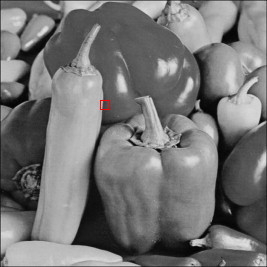
\includegraphics[width=0.45\textwidth]{figures/10/poivrons_grey.png}
        }
        \subfloat[zoom sur le carré rouge]{
            
\includegraphics[width=0.45\textwidth]{figures/10/poivrons_window_grey.png}
        }
    \end{center}
    \caption{Une image est une grille de pixels}
    \label{fig:grid-of-pixel}
\end{figure}

Une image est donc naturellement représentée par une matrice $ M $ d'entiers entre $ 0 $ et $ 255 $. Nous allons utiliser les matrices de \texttt{numpy} pour représenter et manipuler les images. En python, le coin en haut à gauche de l'image correspond au coefficient \texttt{M[0, 0]} de la matrice, comme en mathématiques. Mais attention, comme en mathématiques, le premier indice correspond à l'axe des $ y $ et le second à l'axe des $ x $. On essaye de toujours avoir \autoref{fig:convention-image} en tête. Moyen mnémotechnique : les pixels sont organisés comme lorsqu'on \mintinline{python}{print(M)}.

\begin{figure}[h!]
    \begin{center}
        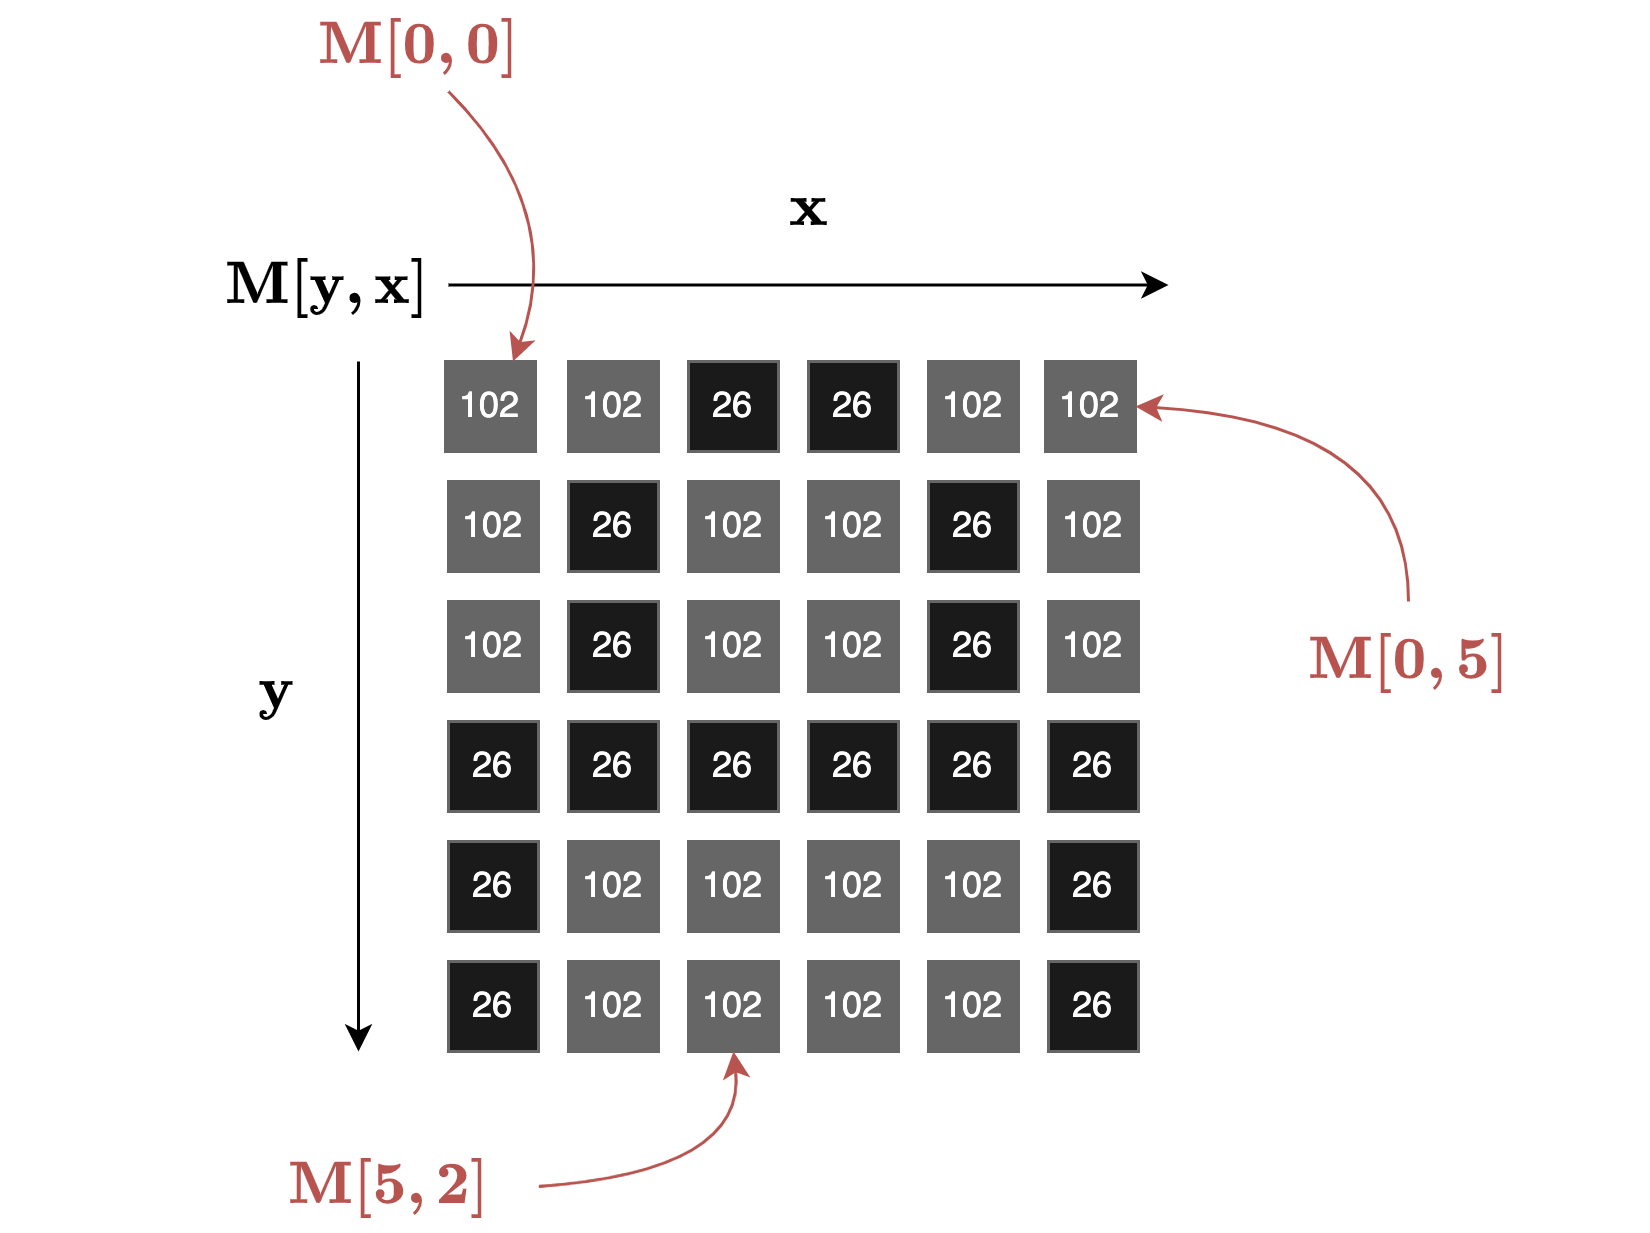
\includegraphics[width=0.65\textwidth]{figures/10/image_grise.png}
    \end{center}
    \caption{ Convention image}
    \label{fig:convention-image}
\end{figure}

\subsection*{Importer, affichage, manipuler, sauver}

\paragraph*{Modules utiles} On utilise le module \texttt{PIL} pour ouvrir, sauvegarder et afficher des images. On utile \texttt{numpy} pour les manipuler.

Écrire dans la console de \texttt{pyzo}
\begin{verbatim}
    pip install Pillow
\end{verbatim}

Puis on écrit en début de fichier 
\begin{minted}{python}
    from PIL import Image
    import numpy as np
\end{minted}

\paragraph*{Importer une image} Téléchargez l'image à l'adresse \href{https://cutt.ly/T4j2eT6}{https://cutt.ly/T4j2eT6} et enregistrez là dans le même dossier que votre fichier python de travail, au nom \texttt{poivrons.png}. Vous pouvez aussi utiliser vos propres images si vous le souhaitez. On peut l'importer dans python avec
\begin{minted}{python}
    img = Image.open('poivrons.png')
\end{minted}

\paragraph*{Afficher une image} On une utilise la méthode \texttt{show()}:
\begin{minted}{python}
    img.show()
\end{minted}

\paragraph*{Obtenir la valeur des pixels sous la forme d'un tableau \texttt{numpy}} Il faut convertir l'image en tableau numpy \emph{et le copier}, sinon on ne peut pas modifier les pixels.
\begin{minted}{python}
    img_grey = img.convert('L') # conversion en image grise
    arr = np.asarray(img_grey).copy()
\end{minted}

\paragraph*{Repasser d'un tableau \texttt{numpy} à une \texttt{Image}}
\begin{minted}{python}
    img = Image.fromarray(arr)
\end{minted}

\paragraph*{sauvegarder une \texttt{Image}}
\begin{minted}{python}
    img.save('poivrons_gris.png', format='PNG')
\end{minted}

\ques Vérifiez que vous arrivez à exécuter les étapes ci-dessus pour finalement produire une version grise de l'image \texttt{poivrons.png}.

\subsection*{Manipulation basique d'image}

\ques Créez les images \autoref{fig:basic-manipulation}

\begin{figure}[!h]
    \begin{center}
        \subfloat[Image mirroir]{
            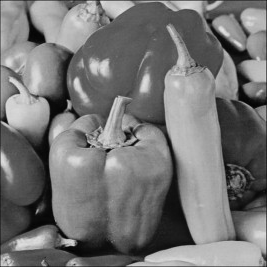
\includegraphics[width=0.3\textwidth]{figures/10/miroir.png}
        }
        \subfloat[Image en négatif]{
            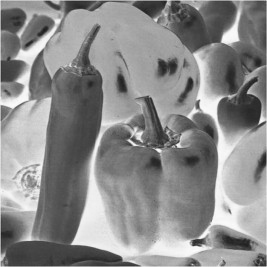
\includegraphics[width=0.3\textwidth]{figures/10/negatif.png}
        }
        \subfloat[Moitié gauche]{
            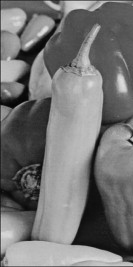
\includegraphics[width=0.15\textwidth]{figures/10/moitie_gauche.png}
        }
    \end{center}
    \caption{Manipulations basiques d'images}
    \label{fig:basic-manipulation}
\end{figure}

\subsection*{Jeu sur la luminosité}

Le but de cette question est d'éclaircir une image. Pour éclaircir une image, il faut globalement augmenter la valeur des pixels. Mais attention, on ne peut pas juste ajouter une constante car la valeur des pixels ne doit pas dépasser 255. À la place, il faut trouver une fonction \[
    eclair:
    \begin{cases}
        [0, 255] &\rightarrow [0, 255]\\
        pixel &\mapsto \quad ?
    \end{cases}
\]
telle que $ eclair(x) \geq x $.

\quessques Donner une fonction qui ressemble à celle \autoref{fig:eclair-func}

\begin{figure}[h!]
    \begin{center}
        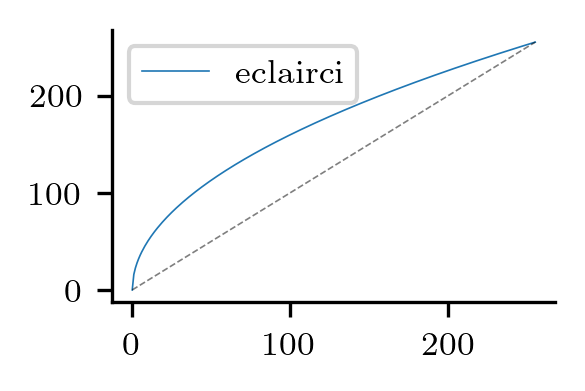
\includegraphics[width=0.4\textwidth]{figures/10/eclair_func.png}
    \end{center}
    \caption{Fonction d'éclaircissement}
    \label{fig:eclair-func}
\end{figure}

\ssques Appliquer la fonction à chaque pixel de l'image et vérifier qu'on obtient une image éclaircie, similaire à \autoref{fig:img-eclaircie}. Attention, par défaut lorsqu'on lit une \texttt{Image} dans un tableau \texttt{numpy}, les valeurs sont de type \texttt{np.uint8}, c'est à dire des entiers de $ [\![0, 255]\!] $ et les calculs se font alors dans $ \Z / 256 \Z $. Pour sortir de ce mode de calcul, il faut faire une conversion explicite vers \texttt{np.float64} en début de calcul, puis reconvertir en \texttt{np.uint8} à la fin des calculs.

\begin{minted}{python}
    arr = arr.astype(np.float64)
    ... # opérations sur arr
    arr = arr.astype(np.uint8)
\end{minted}

\begin{figure}[h!]
    \begin{center}
        \subfloat[Image éclaircie]{
            \label{fig:img-eclaircie}
            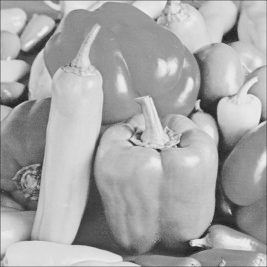
\includegraphics[width=0.4\textwidth]{figures/10/eclairci.png}
        }
        \subfloat[Image assombrie]{
            \label{fig:img-assombrie}
            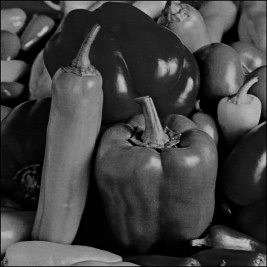
\includegraphics[width=0.4\textwidth]{figures/10/noirci.png}
        }
    \end{center}
    \caption{Changement de luminosité}
\end{figure}

\ssques Trouver une transformation pour obtenir une image cette fois-ci assombrie, comme \autoref{fig:img-assombrie}.

\subsection*{Jeu sur les contrastes}

Une image est très contrastée lorsque les zones sombres sont très sombres et les zones claires très claires, c'est-à-dire que l'ensemble des valeurs des pixels a une grande variance. À l'inverse, une image est peu contrastée si elle est globalement grise, c'est-à-dire que l'ensemble des valeurs des pixels a une faible variance. 


\quessques Trouver deux fonctions dont le graphe ressemble à ceux \autoref{fig:contraste-funcs}

\begin{figure}[h!]
    \begin{center}
        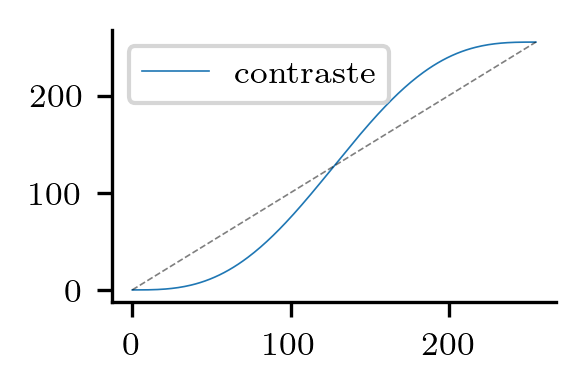
\includegraphics[width=0.4\textwidth]{figures/10/contraste_func.png}
        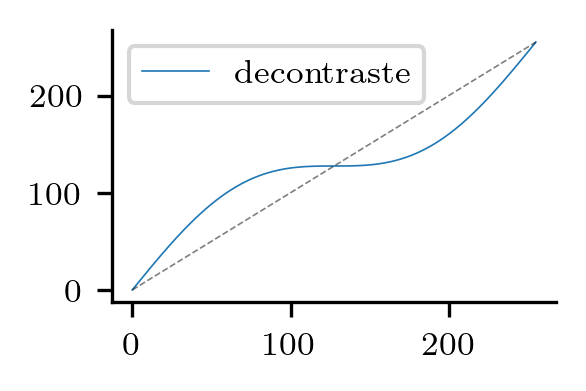
\includegraphics[width=0.4\textwidth]{figures/10/decontraste_func.png}
    \end{center}
    \caption{Fonctions de contrastes}
    \label{fig:contraste-funcs}
\end{figure}

\ssques Recréer les images \autoref{fig:contraste-imgs}

\begin{figure}[h!]
    \begin{center}
        \subfloat[Image contrastée]{
            \label{fig:img-contrast}
            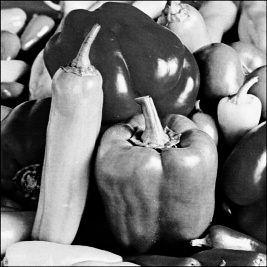
\includegraphics[width=0.4\textwidth]{figures/10/contraste.png}
        }
        \subfloat[Image peu contrastée]{
            \label{fig:img-low-contrast}
            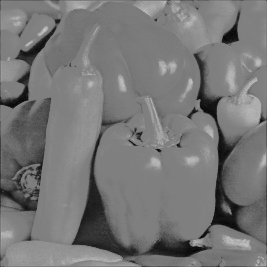
\includegraphics[width=0.4\textwidth]{figures/10/decontraste.png}
        }
    \end{center}
    \caption{Changement de contrastes}
    \label{fig:contraste-imgs}
\end{figure}


% \section*{Représenter la couleur}
% \paragraph*{Qu'est-ce qu'une image en informatique ?} En informatique, une image est un ensemble structuré de pixels. On représente une image par une matrice contenant la valeur de chacun de ses pixels. Traditionnellement, un pixel est un triplet de valeur $ (r, g, b) $ représentant la quantité de rouge $ r $, la quantité de vert $ g $ et la quantité de bleu $ b $. D'ailleurs si vous prenez une loupe et zoomez sur votre écran (d'ordinateur ou de téléphone), vous pourrez voir apparaître des diodes individuelles rouges, vertes et bleues. Ce phénomène peut aussi avoir lieu en déposant une goutte d'eau sur l'écran.

%! TEX root = ../main.tex

\titre{Images et matrices de pixels}

\section*{Transformations locales}

\subsection*{Flou}

Que fait-on mathématiquement lorsqu'on 'floute' une image ? Flouter correspond informellement à répartir la valeur d'un pixel parmi ses voisins. Si $ M $ est une image, on obtient $ M' $ sa version floutée en assignant au pixel $ (i,j) $  une moyenne des pixels autour de $ (i,j) $ dans $ M $:\[
    M'[i, j] = \frac{1}{\#\textrm{voisinage}} \sum_{\textrm{$ (x, y) $ voisin de $ (i, j) $}} M[x,y] 
\]
$ M' $ sera plus ou moins floutée selon la définition que l'on donne à "être voisin de". Par exemple, \autoref{fig:floutage}, on décide que $ (x, y) $ est voisin de $ (i,j) $ si $ max(|x-i|, |y-j|) \leq 1 $.

\begin{figure}[h!]
    \begin{center}
        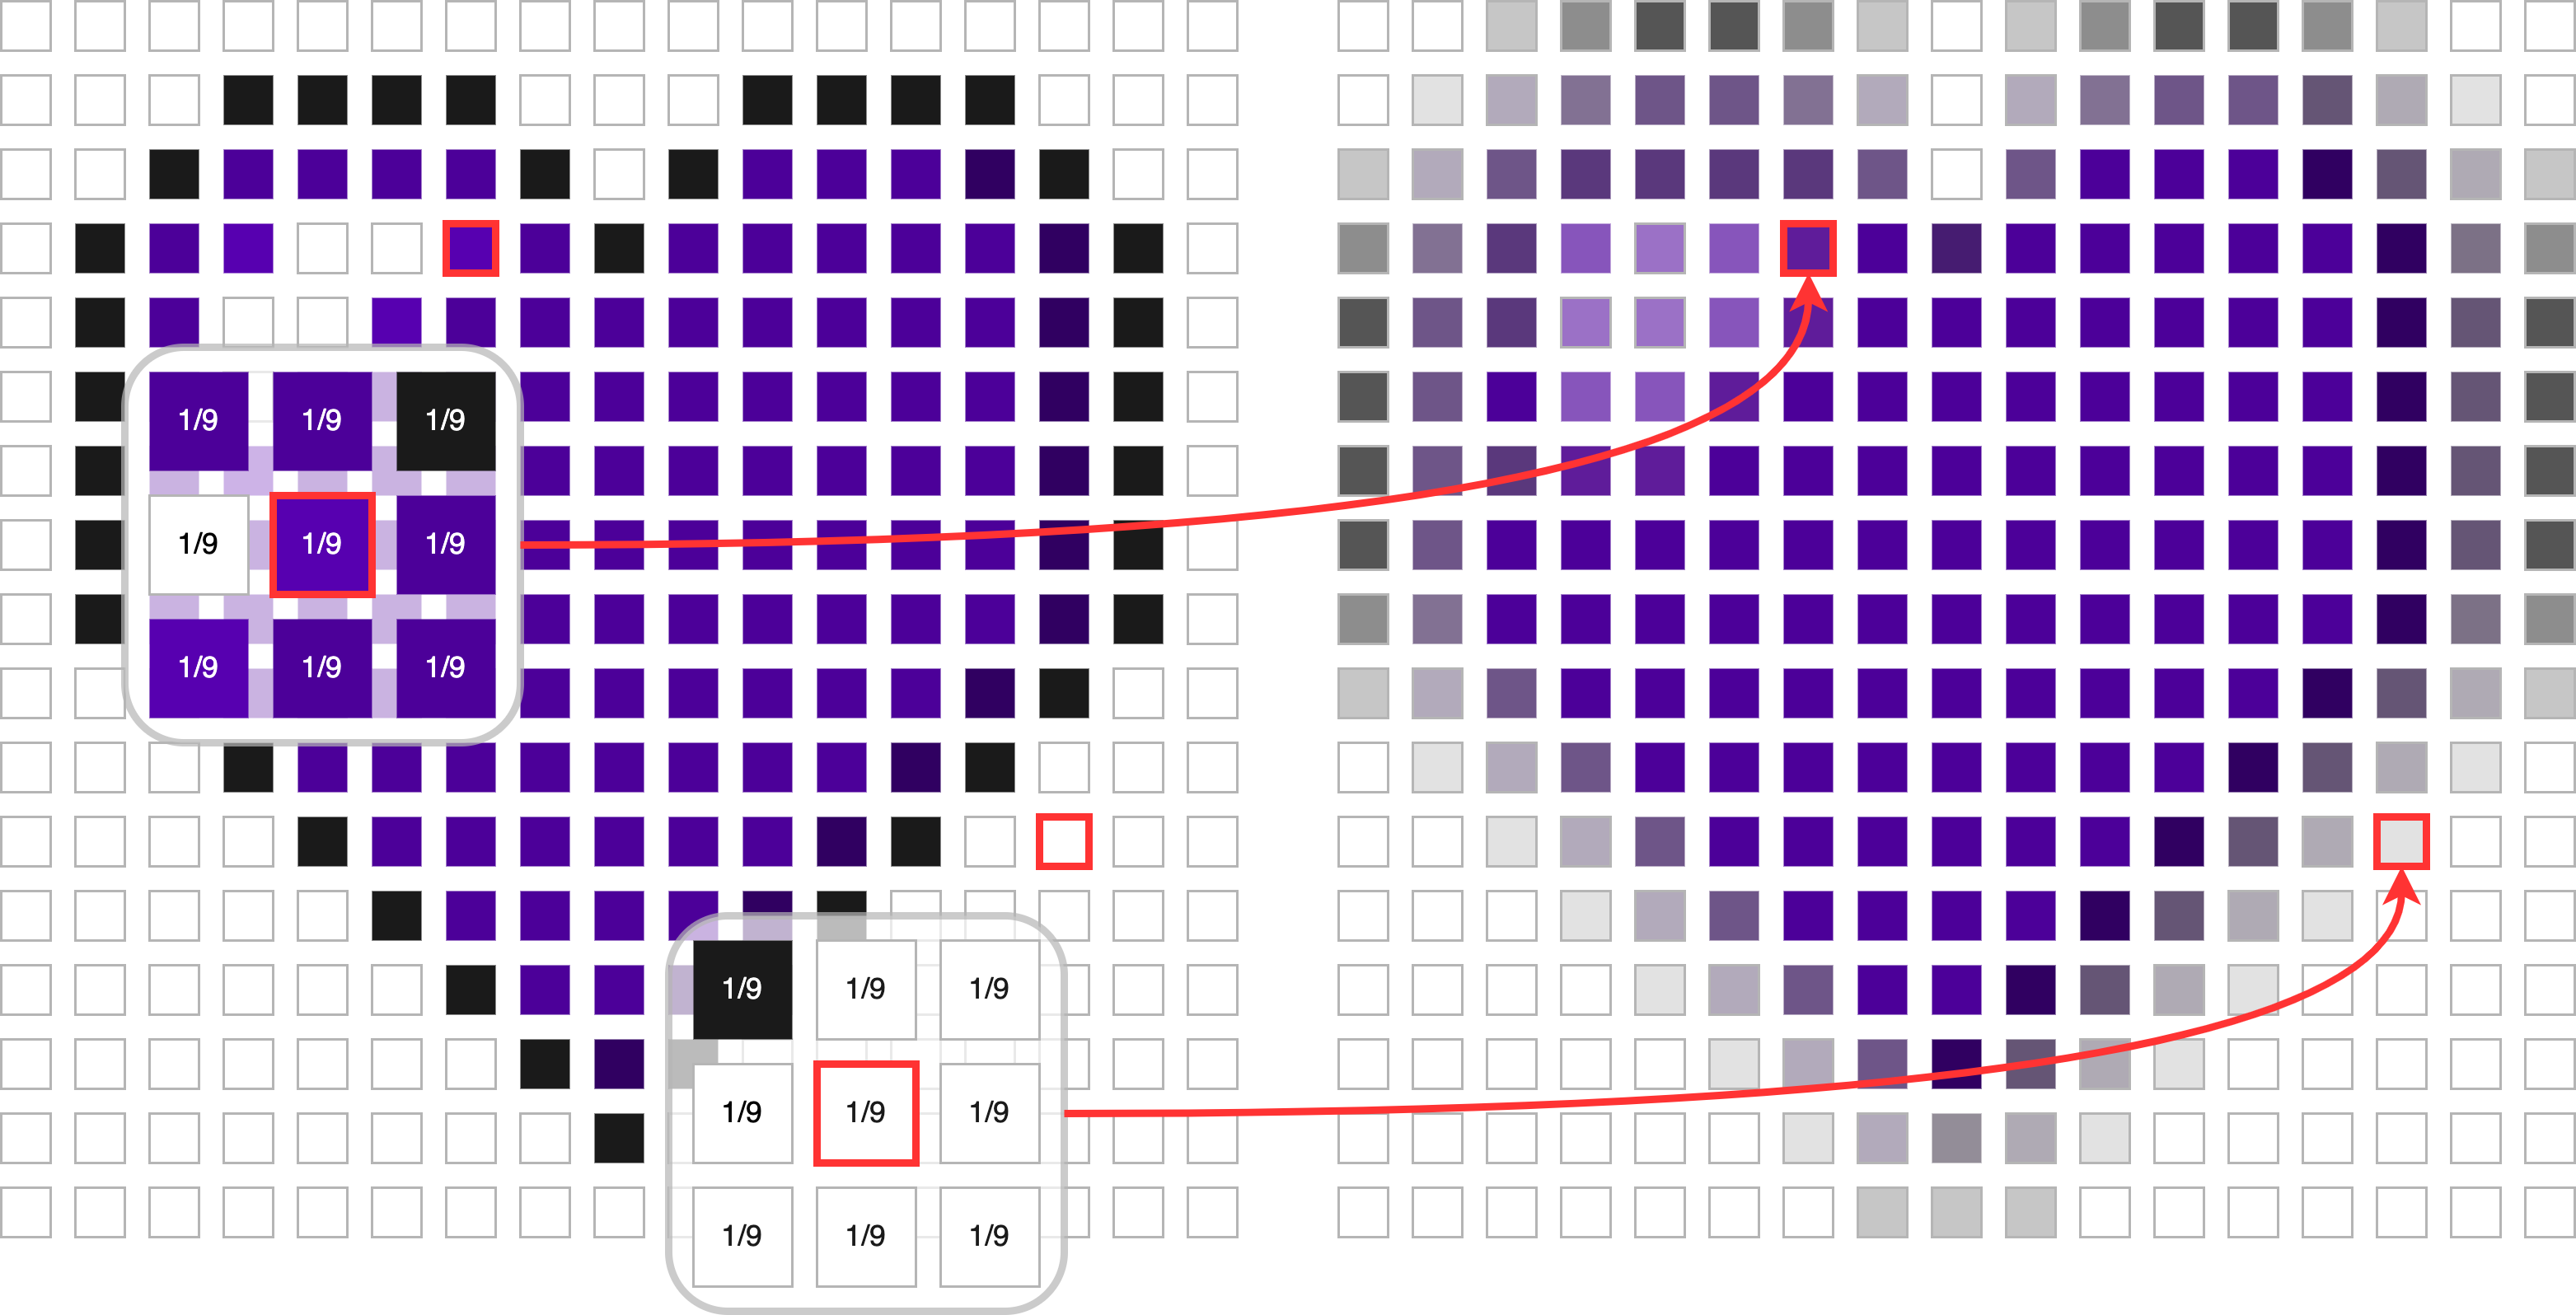
\includegraphics[width=0.9\textwidth]{figures/11/heart-convolution.png}
    \end{center}
    \caption{Floutage sur un voisinage de taille 9}
    \label{fig:floutage}
\end{figure}

\quessques Implémenter l'opération de floutage pour reproduire l'image \autoref{fig:img-blurry}. Attention à bien traiter les pixels du bord de l'image.
\ssques Changer la définition de voisinage en $ max(|x-i|, |y-j|) \leq 4 $ pour obtenir l'image \autoref{fig:img-very-blurry}.

\begin{figure}[h!]
    \centering
    \subfloat[Poivrons flous]{
        \label{fig:img-blurry}
        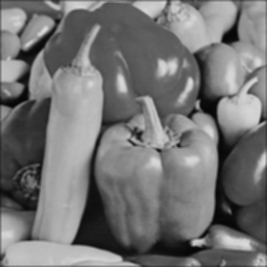
\includegraphics[width=0.45\textwidth]{figures/11/poivrons-blurry.png}
    }
    \subfloat[Poivrons très flous]{
        \label{fig:img-very-blurry}
        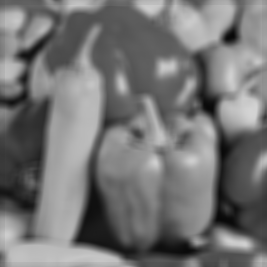
\includegraphics[width=0.45\textwidth]{figures/11/poivrons-very-blurry.png}
    }
    \caption{Transformation en flou}
\end{figure}

\subsection*{Détection de bords}

Une caractéristique de l'opération de floutage est qu'elle ne change pas beaucoup les zones "plates" où tous les pixels sont semblables, mais fait disparaître les bords. On peut considérer qu'une image $ M $ se décompose comme une superposition d'une image $ P $ qui est plate partout, et d'une image $ B $ ne contenant que les bords (c'est un peu comme quand un enfant dessine : d'abord les bords au crayon noir et ensuite la couleur), soit $ M = P + B $. Cette dernière égalité fait réellement intervenir des additions pixel par pixel, i.e. \[
    M[i, j] = P[i, j] + B[i, j]
\]
Alors la fonction $ \phi $ de floutage sélectionne seulement la partie plate : $ \phi(M) = P $. Mais alors on peut récupérer $ B $ ! Il suffit de faire la soustraction $ M - \phi(M) $.

\ques Utiliser les deux images générées à la question précédente pour extraire les images de bords et les visualiser en négatif comme \autoref{fig:edges}. Attention il faut gérer à la main le cas des pixels qui sortent de l'intervalle $ [0, 255] $.

\begin{figure}[h!]
    \begin{center}
        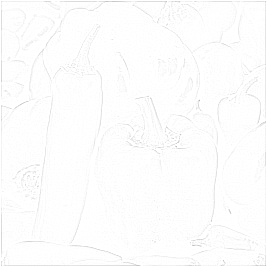
\includegraphics[width=0.45\textwidth]{figures/11/fine-edge-poivrons.png}
        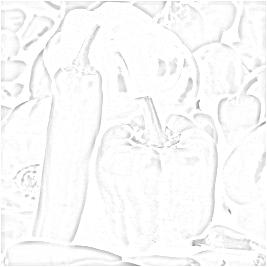
\includegraphics[width=0.45\textwidth]{figures/11/coarse-edge-poivrons.png}
    \end{center}
    \caption{Extraction des bords}
    \label{fig:edges}
\end{figure}


\section*{Représenter la couleur (hors-programme)}

Évidemment, la plupart des images ne sont pas en noir et blanc mais en couleur. Pour représenter un pixel d'une couleur, il ne faut plus un seul nombre mais 3, $ r $, $ g $ et $ b $, qui représentent respectivement le niveau de rouge, le niveau de vert et le niveau de bleu. À nouveau, chaque valeur évolue entre $ 0 $ et $ 255 $. Par exemple, un pixel de valeur \texttt{[0, 255, 255]} représente la couleur cyan (vert + bleu).

Si vous regardez de très près les pixels qui composent vos écrans d'ordinateur ou de téléphone, en utilisant une loupe ou bien en déposant une goutte d'eau sur l'écran, vous pourrez d'ailleurs voir des diodes rouges vertes et bleues, utilisées pour donner l'illusion de couleur.

Ainsi, une image en couleur est représentée par une matrice de pixels, où chaque pixel contient trois valeurs. Si l'image est de hauteur $ h $ et de largeur $ w $, sa matrice de représentation est donc de dimension $ h \times w \times 3 $.

Dans la suite on pourra utiliser les fonctions suivantes pour n'avoir à manipuler que des tableaux numpy:

\begin{minted}{python}
    def load_as_rgb_array(name):
        img = Image.open(name).convert('RGB')
        return np.asarray(img).copy()

    def save_rgb_array_as_img(array, name):
        img = Image.fromarray(array.astype(np.uint8), mode='RGB')
        img.save("{}.png".format(name), format='PNG')
\end{minted}

\quessques Quelle est la dimension de la matrice représentant une image $ 100 \times 100 $

\quessques Créer trois images \texttt{red.png}, \texttt{green.png} et \texttt{blue.png} de taille $ 100 \times 100 $ et représentant respectivement un carré rouge, un carré bleu et un carré vert.

\ssques Comment représenter le noir et le blanc dans les images en couleur ? Recréer l'image \autoref{fig:rgb-squares}, qui est de taille $ 100 \times 100 $.

\begin{figure}[h!]
    \begin{center}
        
\includegraphics[width=0.4\textwidth]{figures/11/rgb-squares.png}
    \end{center}
    \caption{Les couleurs primaires et le blanc}
    \label{fig:rgb-squares}
\end{figure}

\ssques Quelle est la différence entre un pixel \texttt{[0, 0, 255]} et un pixel \texttt{[0, 0, 100]}.

\quessques Recréer l'image \autoref{fig:venn-couleur}, qui est de taille $ 100 \times 100 $ et où les cercles sont de diamètres $ 50 $ pixels.

\begin{figure}[h!]
    \begin{center}
        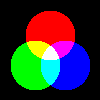
\includegraphics[width=0.4\textwidth]{figures/11/rgb-venn.png}
    \end{center}
    \caption{Diagramme de Venn des couleurs}
    \label{fig:venn-couleur}
\end{figure}


%! TEX root = ../main.tex

\titre{Le language de requête SQL}

\section{Requêtes SQL}

\subsection{{Bases de données relationnelles}}

Comment organiser et interagir avec des giganstesques quantité de données ? Cette question est à l'origine d'un champ crucial de l'informatique : les \textit{systèmes de gestion de bases de données} (SGBD). Un SGBD est un logiciel dont la charge est précisément de stocker, organiser et accéder à un ensemble de données. Leur fonctionnement est extrêmement complexe, nous nous contenterons d'apprendre à \textit{interagir} avec ces systèmes, par le biais du langage SQL (pour \textit{Structured Query Language}).


Plus précisément, nous nous intéressons au bases de données dites \textit{relationnelles} (BDR). Schématiquement, les bases de données relationnelles sont composées de plusieurs \textit{tables} (sorte d'équivalent des tableaux bidimensionnels d'Excel), et de \textit{relations} entre ces tables. Par exemple, dans la base de données \textsc{Mondial} (voir le site \href{The MONDIAL Database}{https://www.dbis.informatik.uni-goettingen.de/Mondial/}), qui contient pléthore d'informations géographiques et socio-économiques à l'échelle mondiale, on trouve une table \texttt{country} qui contient 6 \textit{attributs}, voir \autoref{tab:country}


\begin{table}[h!]
	\centering
	\begin{tabular}{|cccccc|}
		\hline
		\texttt{Name} & \texttt{Code}$ \star $ & \texttt{Capital} & \texttt{Province} & \texttt{Area}                        & \texttt{Population} \\
		              &                        &                  &                   & Surface du pays en $ \textrm{km}^2 $ &                     \\
		\hline
	\end{tabular}
	\caption{la table \texttt{country} }
	\label{tab:country}
\end{table}

Un attribut est simplement le nom donné à une des colonnes de la table. Un \textit{enregistrement}, ou \textit{entrée}, est une ligne de la table. Par exemple, voici les 3 premiers enregistrements de la table \texttt{country}
\begin{table}[h!]
	\centering
	\begin{tabular}{|cccccc|}
		\hline
		\texttt{Name} & \texttt{Code}$ \star $ & \texttt{Capital} & \texttt{Province} & \texttt{Area} & \texttt{Population} \\ \hline
		Albania       & AL                     & Tirana           & Albania           & 28750         & 281977              \\
		Greece        & GR                     & Athina           & Attixis           & 131940        & 10432481            \\
		Cyprus        & CY                     & Nicosia          & Cyprus            & 9251          & 918100              \\ \hline
	\end{tabular}
	\caption{3 premiers enregistrements de la table \texttt{country} }
	\label{tab:country}
\end{table}

En général, une table contient un grand nombre d'enregistrements et l'utilisateurs connaît uniquement le nom des attributs de la table (il y a trop d'enregistrements pour tous les regarder individuellement).

\subsubsection*{Clefs primaires}
Que veut dire le symbole $ \star $ à côté de l'attrubut \texttt{Code} ? C'est une indication pour signifier que l'attribut \texttt{Code} forme la clef primaire de la table \texttt{country}, c'est-à-dire que chaque enregistrement de la table possède une valeur pour \texttt{Code} distincte (il n'y a pas de doublons). Ainsi, la valeur de \texttt{Code} permet d'identifier \textit{uniquement} un enregistrement de la table ; par exemple GR identifie uniquement la seconde entrée de \texttt{country}.

En général, la clef primaire est constituée d'un seul attribut -- mais ce n'est pas obligatoire. Par exemple, il existe une table \texttt{encompasses}, toujours dans la base de données \textsc{Mondial}, dont la clef primaire est le couple d'attributs \texttt{(Country, Continent)} -- voir \autoref{tab:encompasses}. La table \texttt{encompasses} indique pour chaque pays les continents dans lequel se trouve le pays et la pourcentage de la surface du pays dans chacun de ces coninents. L'attribut \texttt{country} seul n'est pas une clef primaire car il est possible qu'un pays soit à cheval sur plusieurs continents (par exemple la Russie, représentée par un "R" dans la table).


\begin{table}[h!]
	\begin{tabular}{|ccc|}
		\hline
		\texttt{Country}$ \star $                 & \texttt{Continent}$ \star $ & \texttt{Percentage}                                 \\
		Clef étrangère pour \texttt{country.Code} &                             & Pourcentage de la surface du pays dans le continent \\ \hline
		R                                         & Europe                      & 23.15                                               \\
		R                                         & Asia                        & 76.85                                               \\
		RA                                        & South America               & 100                                                 \\
		RB                                        & Africa                      & 100                                                 \\ \hline
	\end{tabular}
	\caption{4 premières entrées de la table \texttt{encompasses}}
	\label{tab:encompasses}
\end{table}
\subsubsection*{Clef étrangère}

Dans la table \texttt{encompasses}, vous aurez peut être remarqué que \texttt{Country} est une "clef étrangère pour \texttt{country.Code}". Qu'est-ce que cela signifie ?

Tout l'intérêt des bases de données relationnelles est de considérer les tables non pas individuellement mais comme un ensemble lié par des relations. Une clef étrangère permet de mettre en correspondance les lignes d'une table avec les lignes d'une autre table, en mettant en relation la clef étrangère de la première avec la clef primaire de la seconde. En l'occurrence, cela signifie simplement qu'un enregistrement de la table \texttt{encompasses} dont l'attribut \texttt{Country} est, par exemple, FR évoque le même pays que l'enregistrement de \texttt{country} dont l'attribut \texttt{Code} est FR.

Cela nous permettra par exemple de créer une grande table rassemblant à la fois les informations de \texttt{Country} et \texttt{Code}, appelée une \textit{jointure}. Une image vallant mille mots, regarder \autoref{fig:jointure}. Une telle table pourra être utile pour par exemple répondre à la question "Quelle est la surface totale d'Europe?".

\begin{figure}[h]
	\begin{center}
		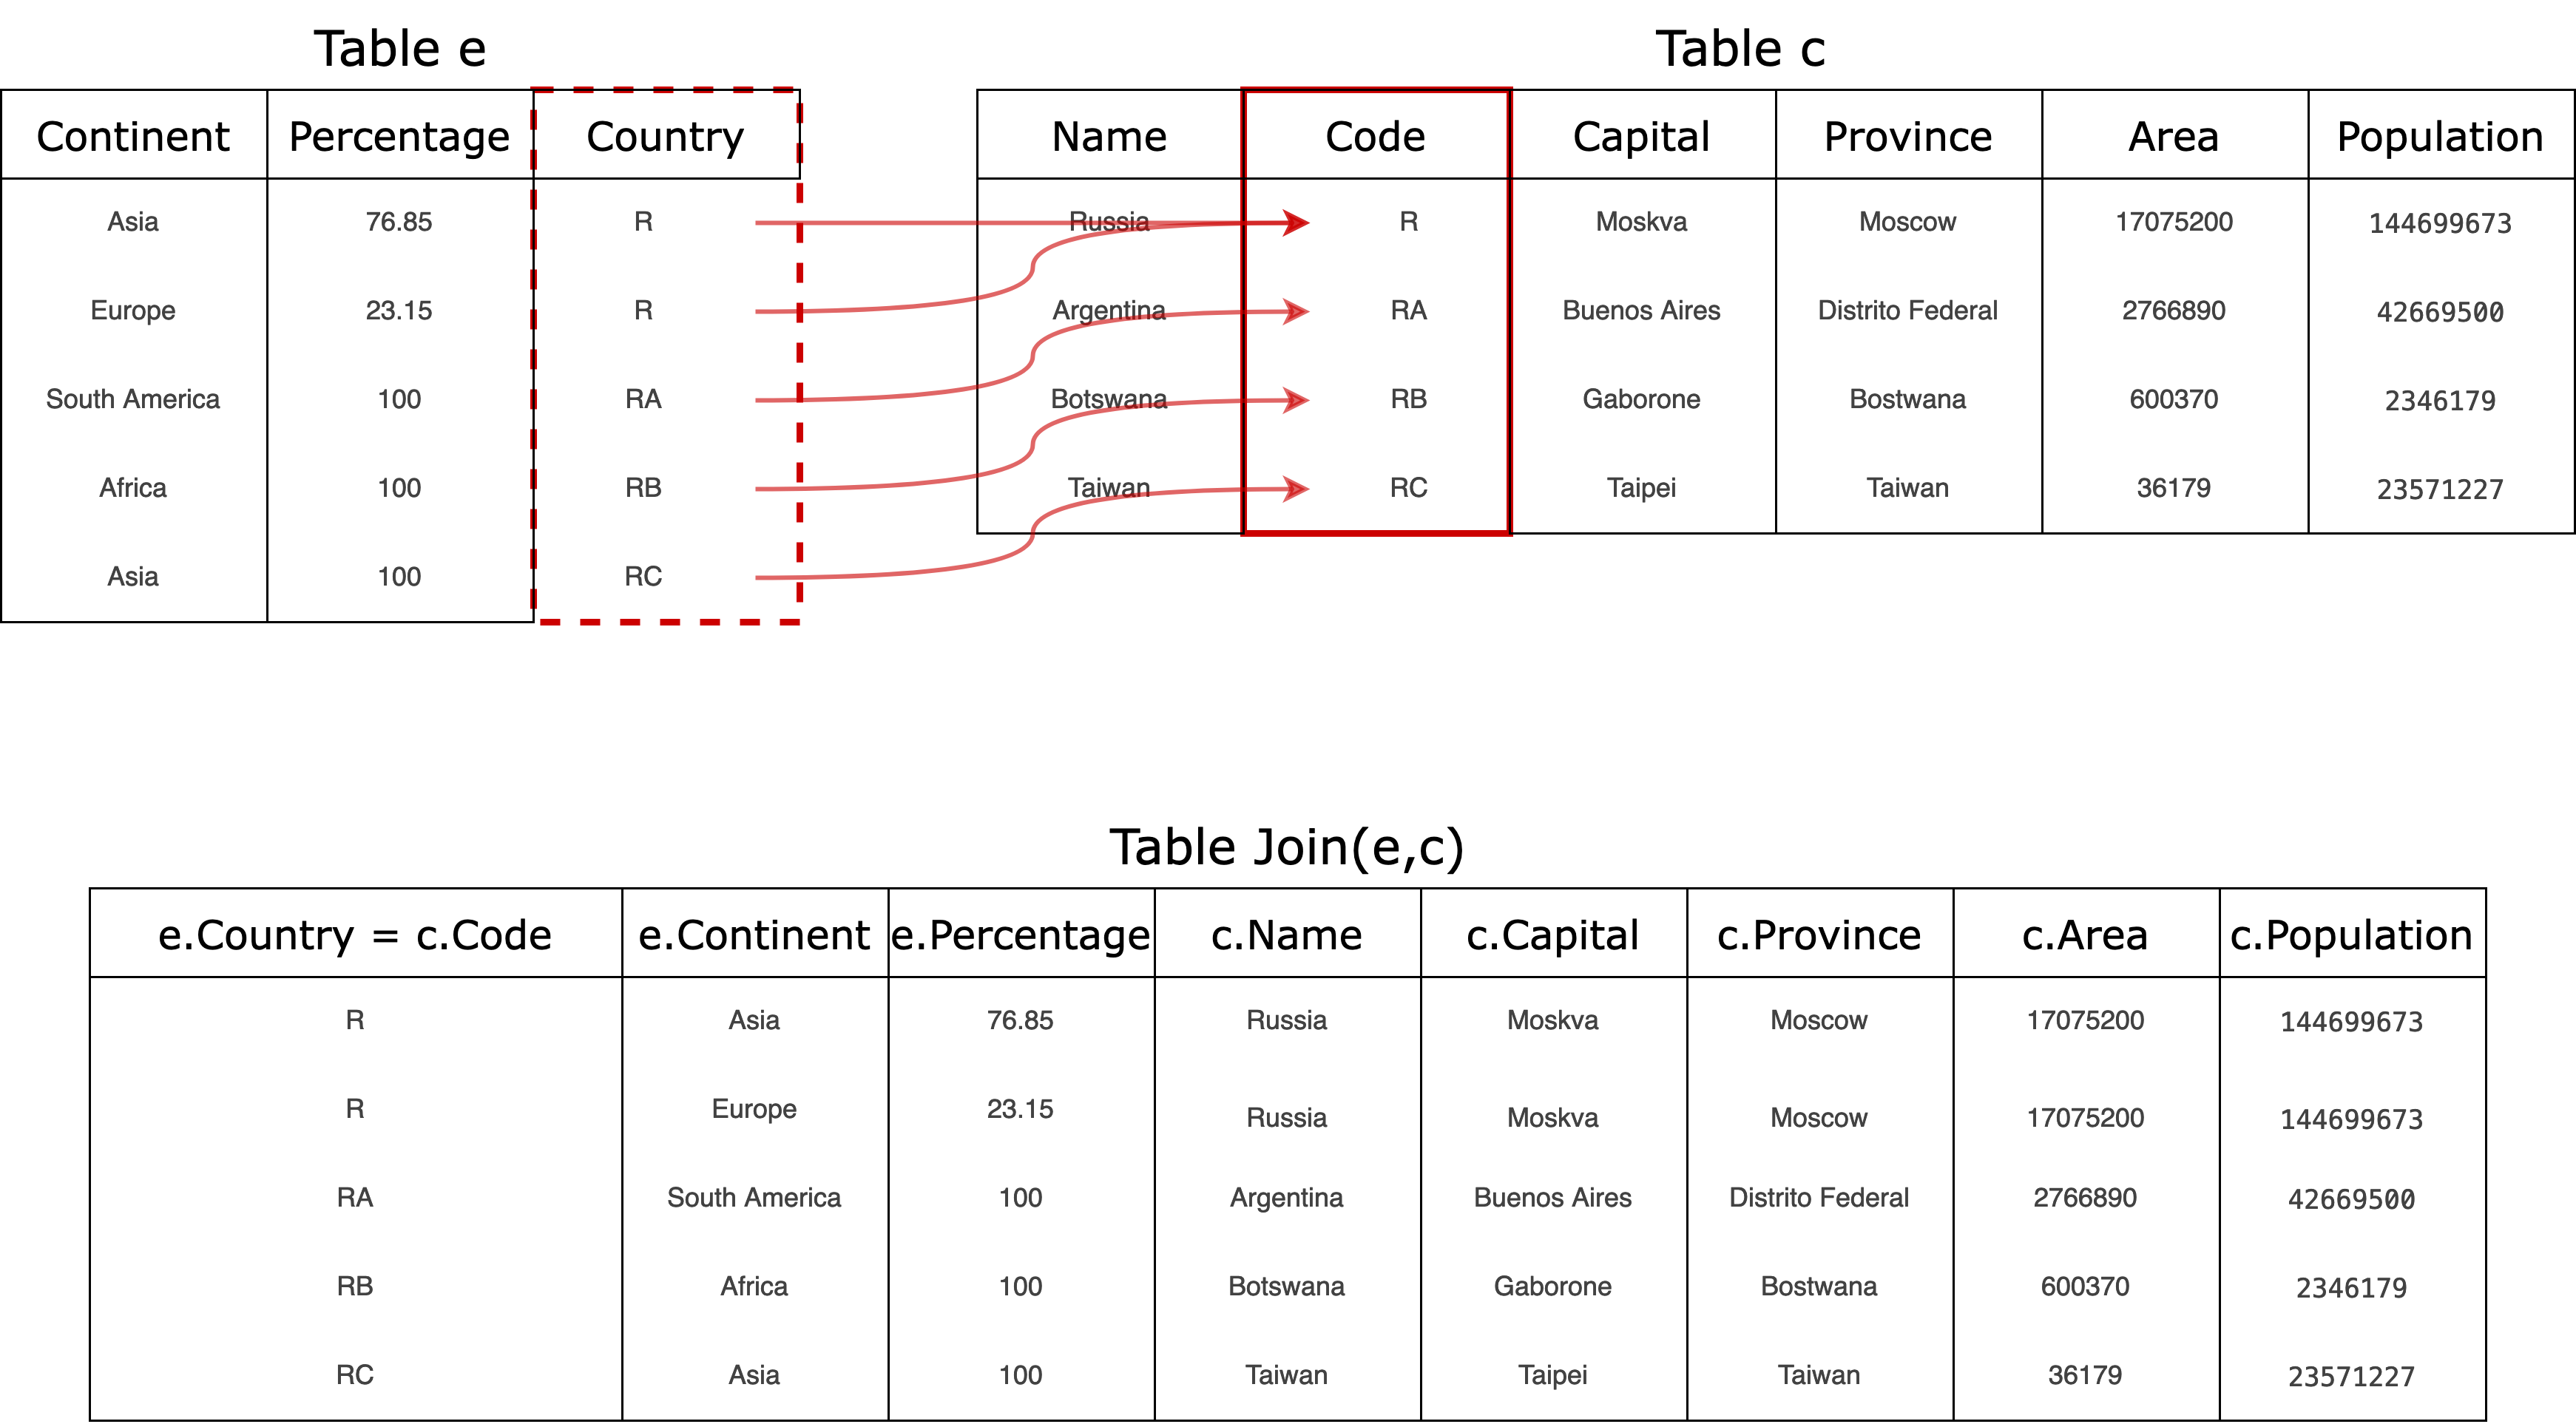
\includegraphics[width=0.95\textwidth]{figures/12/bddr-mondial.png}
	\end{center}
	\caption{Jointure de \texttt{encompasses} et \texttt{country} sur $ \texttt{encompasses.Country} = \texttt{country.Code} $ }
	\label{fig:jointure}
\end{figure}


\subsection{Le language SQL}

Comme mentionné avant, le language SQL permet d'interagir avec le système de base de données : manipuler des tables, extraire des enregistrements, sélectionner certains attributs, faire des jointures, etc. On opte ici par une présentation du language par l'exemple, en augmentant petit à petit le niveau de difficulté.

\subsubsection*{Pour tester ses requêtes en ligne}

Il pourra être utile de tester les requêtes réellement sur la base de données \textsc{Mondial}. Pour cela, suivre les instructions suivantes :
\begin{enumerate}
	\item aller sur la page \href{https://sqliteonline.com/}{https://sqliteonline.com/}.
	\item cliquer sur \texttt{Import} dans la barre d'outils du haut et importer le fichier de base de données que vous pouvez télécharger à l'adresse \href{https://gabriel.belouze.com/tps/data/bdd-mondial.sql}{https://gabriel.belouze.com/tps/data/bdd-mondial.sql}, qui crée le sous-ensemble de \textsc{Mondial} avec lequelle on va travailler.
	\item  cliquer sur OK. Vous devriez voir apparaître dans la barre de gauche les tables \texttt{Country}, \texttt{City}, \texttt{Economy}, \texttt{Encompasses}, \texttt{Spoken}.
\end{enumerate}

Ensuite, il suffit d'écrire les requêtes dans l'éditeur de texte et de les tester avec le bouton \texttt{Run}.

\subsubsection{Premiers pas}

Regardons juste l'attribut \texttt{Name} de la table \texttt{country}.

\begin{minted}{sql}
    SELECT Name FROM country;
\end{minted}

Remarquez que les requêtes SQL se terminent par un point virgule. Remarquez également que SQL ne fait pas la différence entre minuscules et majuscules, on aurait tout aussi bien pu écrire

\begin{minted}{sql}
    SeleCt NAMe froM COUNTry;
\end{minted}

Traditionnellement, les mots clefs (ici \mintinline{sql}{SELECT} et \mintinline{sql}{FROM}) sont écrits tout en majuscules.

Regardons les attributs \texttt{Area} et \texttt{Population} de la table \texttt{country}
\begin{minted}{sql}
    SELECT Area, Population FROM Country;
\end{minted}

Remarque : contrairement à \texttt{Python}, les espaces, retours à la ligne et indentations ne sont pas importants en SQL. On aurait tout aussi bien pu écrire
\begin{minted}{sql}
    SELECT
                    Area,
                Population             FROM 

        Country
    ;
\end{minted}

Mais évidemment, une bonne indentation clarifiera la lecture et relecture de vos requêtes.

\quessques Écrire une requête pour obtenir les pays du monde et leurs capitales.
\ssques Écrire une requête pour obtenir toute la table \texttt{country}

\paragraph*{} Lorsque l'on veut récupérer l'intégralité d'une table, il devient pénible de devoir écrire le nom de tous les attributs. SQL permet de mettre le symbole \mintinline{sql}{*} à la place. Ainsi, votre dernière requête aurait pu s'écrire

\begin{minted}{sql}
    SELECT * FROM Country;
\end{minted}

\paragraph*{} On peut supprimer les doublons avec le mot clef \mintinline{sql}{DISTINCT}. Par exemple, on obtient tous les continents avec la requête 

\begin{minted}{sql}
    SELECT DISTINCT continent FROM encompasses;
\end{minted}

\paragraph*{Conditions} La requête suivante répond à la question : quels sont les pays de plus de 100 000 000 habitants ?

\begin{minted}{sql}
    SELECT Name FROM Country WHERE Population > 100000000;
\end{minted}

On peut créer des conditions plus complexes grâce aux opérateurs \mintinline{sql}{OR} et \mintinline{sql}{AND}, par exemple voici une requête pour trouver les petits pays (de surface inférieure à 50 000 $ \textrm{km}^2 $) mais à grande densité de population (plus que 600 habitants par $ \textrm{km}^2 $).

\begin{minted}{sql}
    SELECT Name
        FROM Country
        WHERE Area < 50000 AND Population / Area > 600;
\end{minted}


\paragraph*{Tri du résultat} On peut aussi obtenir la même liste mais triée dans l'ordre croissant

\begin{minted}{sql}
    SELECT Name 
        FROM Country 
        WHERE Population > 100000000 
        ORDER BY Name ASC;
\end{minted}

Ou dans l'ordre décroissant

\begin{minted}{sql}
    SELECT Name 
        FROM Country 
        WHERE Population > 100000000 
        ORDER BY Name DESC;
\end{minted}

\paragraph*{Tronquer le résultat} On peut limiter le nombre de résultat avec la syntaxe \mintinline{sql}{LIMIT n}, où \texttt{n} est un entier. On peut aussi ignorer les \texttt{m} premiers enregistrements du résultat avec la syntaxe \mintinline{sql}{OFFSET m}. Par exemple, la requête suivante trouve les 5 premiers pays (pour l'ordre alphabétique) dont la population dépasse 100M

\begin{minted}{sql}
    SELECT Name
        FROM Country
        WHERE Population > 100000000
        ORDER BY Name ASC
        LIMIT 5;
\end{minted}

et les 3 suivants

\begin{minted}{sql}
    SELECT Name
        FROM Country
        WHERE Population > 100000000
        ORDER BY Name ASC
        LIMIT 3
        OFFSET 5;
\end{minted}

\ques Rédiger une requête pour obtenir
\ssques les 3 pays les plus peuplés du monde, avec leur population correspondante.
\ssques le 4e et 5e pays le moins peuplé du monde.


\subsubsection{Jointures}
Jusque là on n'a pu considérer les tables qu'une par une. Comment faire en SQL l'équivalent de ce qui est représenté \autoref{fig:jointure} ? Voici par exemple une requête pour obtenir les pays d'Europe

\begin{minted}{sql}
    SELECT country.Name
        FROM country JOIN encompasses ON country.Code = encompasses.Country
        WHERE encompasses.Continent = "Europe";
\end{minted}

La partie \mintinline{sql}{country JOIN encompasses ON country.Code = encompasses.Country} crée une table similaire à celle représentée \autoref{fig:jointure}, c'est-à-dire dont les attributs sont

\begin{table}[h!]
	\centering
	\begin{tabular}{|ccccc|}
		\hline
		\texttt{country.Name}       & \texttt{country.Code}        & \texttt{country.Capital}       & \texttt{country.Province}       & \texttt{country.Area} \\
		\texttt{country.Population} & \texttt{encompasses.Country} & \texttt{encompasses.Continent} & \texttt{encompasses.Percentage} &                       \\
		\hline
	\end{tabular}
\end{table}

et dans laquelle pour chaque enregistrement $ country.Code $ et $ encompasses.Country $ sont égaux.

Pour éviter de devoir écrire le nom complet de la table d'origine, on peut fournir des noms plus courts avec le mot clef \mintinline{sql}{AS}. Ainsi la requête précédente aurait pu s'écrire

\begin{minted}{sql}
    SELECT c.Name
        FROM country AS c JOIN encompasses AS e ON c.Code = e.Country
        WHERE e.Continent = "Europe";
\end{minted}

\ques Rédiger une requête pour obtenir
\ssques les pays du continent américain qui comptent moins de 10 habitants par $ \textrm{km}^2 $.
\ssques les capitales européennes situées à une latitude supérieure à $ 60^{\circ} $.
\ssques les pays ayant plus de 1 000 000 $ \textrm{km}^2 $ dans l'Asie, triés par surface de territoire asiatique décroissante. Donner également la valeur de cette surface de territoire asiatique.

\subsubsection{Fonctions d'agrégation}

SQL donne également accès à des fonctions qui réalisent des calculs sur l'ensemble d'une table, les fonctions d'agrégation. \autoref{tab:important-agregation-func} rassemble les plus importantes de ces fonctions (et celles qqui sont au programme).

\begin{figure}[h!]
	\centering
	\begin{tabular}{|ll|}
		\hline
		\mintinline{sql}{COUNT()} & nombre d'enregistrements      \\
		\mintinline{sql}{MAX()}   & valeur maximale d'un attribut \\
		\mintinline{sql}{MIN()}   & valeur minimale d'un attribut \\
		\mintinline{sql}{SUM()}   & somme d'un attribut           \\
		\mintinline{sql}{AVG()}   & moyenne d'un attribut         \\
		\hline
	\end{tabular}
	\caption{Fonctions d'agrégation}
	\label{tab:important-agregation-func}
\end{figure}

Ainsi la requête suivante calcule le nombre de pays en Asie

\begin{minted}{sql}
    SELECT COUNT(Country) FROM Encompasses WHERE Continent="Asia";
\end{minted}

Puisqu'ici on compte juste le nombre de lignes, la colonne que l'on donne à l'intérieur de \mintinline{sql}{COUNT(...)} n'importe pas. Il est donc plus élégant d'écrire

\begin{minted}{sql}
    SELECT COUNT(*) FROM Encompasses WHERE Continent="Asia";
\end{minted}

\ques Rédiger une requête pour obtenir
\ssques la surface totale du continent \texttt{Africa}.
\ssques la population mondiale.
\ssques la population moyenne par pays.
\ssques le nombre de pays de plus de 1 000 000 de $ \textrm{km}^2 $

% \subsubsection{Groupements}
%
%
% La base de données \texttt{Mondial} possède également une table \texttt{spoken}, décrite \autoref{tab:spoken}.
%
% \begin{table}
% 	\centering
%
% 	\begin{tabular}{|ccc|}
% 		\hline
% 		\texttt{Country}$ \star $                 & \texttt{Language}$ \star $ & \texttt{Percentage}                                      \\
% 		Clef étrangère pour \texttt{country.Code} &                            & Pourcentage de la population du pays qui parle la langue \\
% 		\hline
% 	\end{tabular}
% 	\caption la table \texttt{spoken}
% 	\label{tab:spoken}
% \end{table}
%

% \newpage

%! TEX root = ../main.tex

\titre{Requêtes SQL avancées}


Dans la suite, on dispose des tables décrites \autoref{fig:mondiale}. On marque par $ \star $ les colonnes qui forment la clef primaire de la table.
\begin{figure}[h!]
	\centering
	\subfloat[Table \texttt{country}]{
		\begin{tabular}{|cccccc|}
			\hline
			\texttt{Name} & \texttt{Code}$ \star $ & \texttt{Capital} & \texttt{Province} & \texttt{Area}                        & \texttt{Population} \\
			              &                        &                  &                   & Surface du pays en $ \textrm{km}^2 $ &                     \\
			\hline
		\end{tabular}
	}%
	\qquad
	\subfloat[Table \texttt{encompasses}]{
		\begin{tabular}{|ccc|}
			\hline
			\texttt{Country}$ \star $                 & \texttt{Continent}$ \star $ & \texttt{Percentage}                                 \\
			Clef étrangère pour \texttt{country.Code} &                             & Pourcentage de la surface du pays dans le continent \\
			\hline
		\end{tabular}
	}%
	\qquad
	\subfloat[Table \texttt{city}]{
		\begin{tabular}{|cccccc|}
			\hline
			\texttt{Name}$ \star $ & \texttt{Country}$ \star $                 & \texttt{Province} & \texttt{Population} & \texttt{Longitude} & \texttt{Latitude} \\
			                       & Clef étrangère pour \texttt{country.Code} &                   &                     &                    &                   \\
			\hline
		\end{tabular}
	}%
	\qquad
	\subfloat[Table \texttt{spoken}]{
		\begin{tabular}{|ccc|}
			\hline
			\texttt{Country}$ \star $                 & \texttt{Language}$ \star $ & \texttt{Percentage}                                      \\
			Clef étrangère pour \texttt{country.Code} &                            & Pourcentage de la population du pays qui parle la langue \\
			\hline
		\end{tabular}
	}%
	\qquad
	\subfloat[Table \texttt{economy}]{
		\begin{tabular}{|ccc|}
			\hline
			\texttt{Country}$ \star $                 & \texttt{GDP}                       & \texttt{Agriculture}                        \\
			Clef étrangère pour \texttt{country.Code} & Le PIB en million de dollars       & La part de l'agriculture dans le PIB, en \% \\
			\hline
			\texttt{Service}                          & \texttt{Industry}                  & \texttt{Inflation}                          \\
			La part des services dans le PIB          & La part de l'industrie dans le PIB & Le taux d'inflation                         \\
			\hline
			\texttt{Unemployment}                     &                                    &                                             \\
			Le taux de chômage                        &                                    &                                             \\
			\hline
		\end{tabular}
	}
	\caption{Structure de la base de données \textsc{Mondial}}
	\label{fig:mondiale}
\end{figure}

\section{Agrégations}

SQL permet de regrouper les résultats d'une requête grâce au mot clef \mintinline{sql}{GROUP BY}. Par exemple, on peut regrouper par continent dans la table \textsc{encompasses} en écrivant \mintinline{sql}{GROUP BY Continent}. Ensuite, les fonctions d'agrégation vues au TP précédent permettent de faire des calculs \textit{au sein chaque groupe}. Voici par exemple comment obtenir le nombre de pays de chaque continent 

\begin{minted}{sql}
    SELECT continent, COUNT(*)
        FROM encompasses
        GROUP BY continent;
\end{minted}

Ou encore, avec un exemple plus compliqué, voici comment obtenir la surface totale de chaque continent 

\begin{minted}{sql}
    SELECT e.continent, SUM(c.area * e.percentage)
        FROM encompasses as e JOIN country as c ON c.code = e.country
        GROUP BY e.continent;
\end{minted}

Attention, une fois qu'on regroupe selon une certaine colonne, on ne peut addresser les autres colonnes que par l'intermédiaire des fonctions d'aggrégation. Ainsi la requête suivante \textit{ne veut rien dire et n'est pas correcte} 

\begin{minted}{sql}
    SELECT e.continent, c.name -- NON on ne peut pas sélectionner directement c.name
        FROM encompasses as e JOIN country as c ON c.code = e.country
        GROUP BY e.continent;
\end{minted}

Ensuite, il est possible de filtrer les groupes avec le mot clef \mintinline{sql}{HAVING}. Par exemple, on peut ne sélectionner que les continents d'une surface plus grande que 10 000 000 $ \textrm{km}^2 $ avec 

\begin{minted}{sql}
    SELECT e.continent
        FROM encompasses as e JOIN country as c ON c.code = e.country
        GROUP BY e.continent
        HAVING sum(c.area * e.percentage) > 10000000;
\end{minted}

Notez la différence entre \mintinline{sql}{WHERE} et \mintinline{sql}{HAVING} : le premier filtre \textit{les lignes} avant de former les groupes, et le second filtre \textit{les groupes} après les avoir formés. La forme générale d'une requête est donc 

\begin{minted}{sql}
    SELECT column
        FROM table
        WHERE ligne_condition
        GROUP BY column
        HAVING groupe_condition
\end{minted}

\section{Sous-requêtes}

Le résultat d'une requête est lui-même une table qui peut être elle-même imbriquée dans une nouvelle requête. Par exemple, on peut récupérer la surface moyenne des pays avec la requête 

\begin{minted}{sql}
    SELECT avg(area) FROM country;
\end{minted}

En réutilisant la requête précédente on peut ainsi obtenir les pays dont la surface est plus grande que la moyenne : 

\begin{minted}{sql}
    SELECT name
        FROM country
        WHERE area > (SELECT avg(area) FROM country);
\end{minted}

Les requêtes imbriquées peuvent aussi être utilisées dans la clause \mintinline{sql}{FROM table} à la place de \mintinline{sql}{table}, mais dans cas il faut parfois donner un nom à la table et ses colonnes avec \mintinline{sql}{AS}. Par exemple, la requête suivante compte le nombre de langues parlées dans chaque pays 

\begin{minted}{sql}
    SELECT count(*) FROM spoken GROUP BY country;
\end{minted}

On réutilise cette requête pour obtenir le plus grand nombre de langues parlées dans un seul pays. Notez qu'on donne un nom à la colonne \mintinline{sql}{count(*)} pour pouvoir s'y référer dans le reste de la requête.

\begin{minted}{sql}
    SELECT MAX(n_language)
        FROM (SELECT count(*) as n_language FROM spoken GROUP BY country) as count_table;
\end{minted}

Le mot clef \mintinline{sql}{IN} peut être utilisé pour tester l'appartenance à une table (la table étant, en général, le résultat d'une requête imbriquée). Par exemple, on peut s'inspirer des requêtes ci-dessus pour obtenir le nombre de langues parlées dans les pays \textit{dont la surface est inférieure à la moyenne mondiale} 

\begin{minted}{sql}
    SELECT country, count(*)
        FROM spoken
        WHERE country IN (
            SELECT code
                FROM country
                WHERE area < (SELECT avg(area) FROM country)
        )
        GROUP BY country;
\end{minted}

Vous avez maintenant toutes les clefs pour finir les exercices suivants (les deux premiers sont des rappels du TP précédent). Si vous y arrivez, félicitations vous maîtrisez l'ensemble du programme de SQL de BCPST.

\begin{enonce}[Requêtes de base]
	Rédiger une requête SQL pour obtenir
	\ssques La liste des pays dont la population excède 60M habitants
	\ssques La même liste triée par ordre alphabétique
	\ssques La liste des pays et de leurs populations respectives, triée par ordre croissant de population
	\ssques Le nom des dix pays ayant la plus petite superficie
	\ssques Le nom des dix suivants
\end{enonce}

\begin{enonce}[Jointures]
	Rédiger une requête SQL pour obtenir
	\ssques Le nom des pays qui sont à cheval sur plusieurs continents
	\ssques Les pays du continent américain qui comptent moins de 10 habitants par $ \textrm{km}^2 $
	\ssques Les capitales européennes situées à une latitude supérieure à $ 60^{\circ} $
\end{enonce}

\begin{enonce}[Fonctions d'agrégation]
	\ssques Donner la liste ordonnée des dix langues parlées dans le plus de pays différents.
	\ssques Quelles sont les langues parlées dans exactement 6 pays ? Et de quel pays s'agit-il ?
	\ssques Quelles sont les langues parlées par moins de 30 000 personnes dans le monde ?
	\ssques Quelles sont les 5 langues les plus parlées en Afrique ? Préciser pour chacune d'elle le nombre de personnes qui la parlent.
\end{enonce}

\begin{enonce}[Sous-requêtes]
	\ssques Déterminer les pays majoritairement agricoles dont le taux de chômage est inférieur à la moyenne mondiale.
	\ssques Déterminer pour chaque continent le pays au taux d'inflation le plus faible parmi les pays majoritairement industriels.
    \ssques Déterminer les pays dans lesquels on parle le plus de langues.
    \ssques Quel est le continent le plus riche, en terme de PIB ?
\end{enonce}

%! TEX root = ../main.tex

\titre{Intégration numérique}

Dans ce TP, on s'intéresse au problème du calcul numérique d'une intégrale \[
    I_{a, b}(f) = \int_{a}^{b} f(t)dt
\]
d'une fonction $ f $ continue sur le segment $ [a, b] $. Ce problème intervient régulièrement en physique, mathématiques, biologie, et d'autres domaines encore, lorsqu'il n'est pas possible de calculer une primitive de $ f $, même en ayant recours aux techniques de changements de variable, intégration par partie, et autres techniques d'intégration plus avancées.

Les méthodes que l'on considère se décomposent en deux étapes:
\begin{enumerate}
    \item Une méthode de base pour calculer $ \hat{I}_{u, v}(f) $ une approximation de l'intégrale sur un petit intervalle $ [u, v] $.
    \item Ensuite on utilise la relation de Chasles pour les intégrales: on considère une subdivision régulièrement espacée $ (u_0, u_1, \ldots, u_n) $ de $ [a, b] $ (voir \autoref{fig:subdivision-reguliere}) et on calcule \[
        \hat{I}^{(n)}_{a, b}(f) = \hat{I}_f(u_0, u_1) + \hat{I}_f(u_1, u_2) + \ldots + \hat{I}_f(u_{n-1}, u_n)
    \]
    C'est la généralisation dite \textit{composite} de la méthode de base.
\end{enumerate}

Les méthodes de base auxquelles nous allons nous intéresser sont dites des \textit{de quadrature}, c'est-à-dire qu'elles conduisent à approcher l'intégrale par une somme pondérée finie de valeurs de $ f $ évaluée en différents points. Autrement dit, les méthodes de base calculent une approximation de la forme \[
    \hat{I}_{u, v}(f) = \sum_{k=0}^{p} \alpha_i f(x_i)
\]
où les poids $ \alpha_1, \ldots, \alpha_p $ sont des réels indépendants de $ f $, et les $ x_i $ sont des réels de l'intervalle $ [a, b] $.

L'erreur d'approximation est la différence entre $ I_{a, b}(f) $ et l'approximation de la méthode de base $ \hat{I}_{a, b}(f) $, soit \[
    E_{a, b}(f) =  I_{a, b}(f) -  \hat{I}_{a, b}(f) 
\]

L'erreur d'approximation composite est l'erreur pour l'approximation de la généralisation composite de la méthode de base, soit \[
    E^{(n)}_{a, b}(f) =  I_{a, b}(f) -  \hat{I}^{(n)}_{a, b}(f) 
\]


Enfin, on dira qu'une méthode \textrm{est d'ordre $ k $} lorsque l'erreur d'approximation est nulle si $ f $ est un polynôme de degré inférieur ou égal à $ k $.

On se donne ici la formule pour calculer le $ k $-ième point de la subdivision régulière de $ [a, b] $ de taille $ n $ \[
    u_k = a + k\frac{b-a}{n}, \quad k=0, \ldots, n
\]

\begin{figure}[h!]
    \centering
    \begin{tikzpicture}
        % Segment
        \draw (0,0) -- (6,0);
        \node at (0,0.5) {$a$};
        \node at (6,0.5) {$b$};
        % Ticks and labels
        \foreach \x in {0,...,6}
        {
          \draw (\x,0) -- (\x,-0.2) node[below] {$u_{\x}$};
        }

        % Double-ended arrow
        \draw[<->] (3,0.2) -- (4,0.2) node[midway, above] {$\frac{b-a}{n}$};
    \end{tikzpicture}
    \caption{Subdivision régulière de $ [0, 1] $ de taille $ 5 $}
    \label{fig:subdivision-reguliere}
\end{figure}

\section{Méthode du rectangle}

\subsection{Méthode de base}
La méthode du rectangle est la plus simple : elle consiste à approcher la fonction par une unique valeur qu'elle prend (en général à une des extrêmités de l'intervalle). Ainsi, si l'on choisit l'extrêmité gauche, l'approximation s'écrit \[
    \hat{I}_{u, v}(f) = (v-u) \cdot f(u)
\]
Avec la terminologie vue plus haut, cela revient à prendre $ p=0 $, $ \alpha_0=v-u $ et $ x_0=u $

\quessques Que devient la formule pour $ \hat{I}(u, v) $ si l'on choisit plutôt l'extrêmité droite ?
\ssques Quel est l'ordre de la méthode du rectangle si l'on choisit l'extrêmité gauche ? l'extrêmité droite ?

\begin{figure}[h!]
    \centering
    \begin{tikzpicture}[xscale=5, yscale=3]

        % Area under the constant function
        \fill[blue!20, domain=0.5:1.5, variable=\x]
            (0.5,0)
            -- plot ({\x}, {0.8+0.5*sin(deg(2.5))})
            -- (1.5,0)
            -- cycle;
        % Dotted vertical line
        \draw[dashed] (0.5,0) -- (0.5, {0.8+0.5*sin(deg(2.5)});
        \draw[dashed] (1.5,0) -- (1.5, {0.8+0.5*sin(deg(2.5)});

        % axis
        \draw[-latex] (0,0) -- (2,0) node[below] {$x$};
        \draw[-latex] (0,0) -- (0,2) node[left] {$y$};
        \draw (0.5,0) -- (0.5,-0.1) node[below] {$u$};
        \draw (1.5,0) -- (1.5,-0.1) node[below] {$v$};

        % Constant function
        \draw[blue, line width=1.5pt, domain=0.5:1.5] plot (\x, {0.8+0.5*sin(deg(2.5))});

        % Curve
        \draw[red, line width=1.5pt, domain=0.5:1.5, samples=100] plot (\x, {0.8+0.5*sin(deg(5*\x))}) node[right] {$y=f(x)$};
    \end{tikzpicture}
    \caption{Méthode du rectangle pour l'extrêmité gauche}
    \label{fig:rectangle-method}
\end{figure}

\quessques Écrire une fonction \texttt{rectangle(f, u, v)} qui prend comme argument une fonction \texttt{f}, et des bornes \texttt{u} et \texttt{v}, et renvoie l'approximation de l'intégrale de \texttt{f} entre \texttt{u} et \texttt{v} donnée par la méthode du rectangle. 
\ssques Tester la fonction avec $ \sin(x) $ entre $ 3 $ et $ 4 $. 
\ssques Calculer l'erreur pour l'exemple précédent.


\subsection{Méthode du rectangle composite}

La généralisation composite de la méthode du rectangle applique la méthode du rectangle à chaque subdivision de l'intervalle $ [a, b] $. En utilisant l'extrêmité gauche, cela s'écrit donc
\begin{align*}
    \hat{I}^{(n)}_{a, b}(f) &= \sum_{k=0}^{n-1} f(u_k)(u_{k+1}-u_k)\\
                          &= \frac{b-a}{n}\sum_{k=0}^{n-1} f(a + k \frac{b-a}{n}) 
\end{align*}

C'est essentiellement la forme d'une intégrale de Riemann !

\begin{figure}[h!]
    \centering
    \begin{tikzpicture}[xscale=5, yscale=3]
        % Subdivisions and constant curves
        \foreach \i in {0,1,2,3,4,5} {
            \pgfmathsetmacro{\xa}{0.5 + \i*(1/6)}
            \pgfmathsetmacro{\xb}{0.5 + (\i+1)*(1/6)}
            \fill[blue!20, domain=\xa:\xb, variable=\x]
                (\xa,0) -- plot ({\x}, {0.8+0.5*sin(deg(5*\xa))}) -- (\xb,0) -- cycle;
            \draw[blue, line width=1.5pt, domain=\xa:\xb] plot (\x, {0.8+0.5*sin(deg(5*\xa))});
            \draw[dashed] (\xa,0) -- (\xa, {0.8+0.5*sin(deg(5*\xa))});
            \draw[dashed] (\xb,0) -- (\xb, {0.8+0.5*sin(deg(5*\xa))});
        }

        % Axis and ticks
        \draw[-latex] (0,0) -- (2,0) node[below] {$x$};
        \draw[-latex] (0,0) -- (0,2) node[left] {$y$};
        \draw (0.5,0) -- (0.5,-0.1) node[below] {$u$};
        \draw (1.5,0) -- (1.5,-0.1) node[below] {$v$};

        % Curve
        \draw[red, line width=1.5pt, domain=0.5:1.5, samples=100] plot (\x, {0.8+0.5*sin(deg(5*\x))}) node[right] {$y=f(x)$};

    \end{tikzpicture}

    \caption{Méthode composite du rectangle pour l'extrêmité gauche}
    \label{fig:rectangle-composite-method}
\end{figure}

\quessques Écrire une fonction \texttt{rectangle\_composite(f, a, b, n)} qui calcule l'approximation de l'intégrale de \texttt{f} entre \texttt{a} et \texttt{b} pour la méthode du rectangle composite, avec une subdivision de taille \texttt{n}. On pourra utiliser la fonction \texttt{np.linspace} (cherchez la documentation en ligne pour comprendre comment elle fonctionne).
\ssques Calculer l'erreur avec la même fonction test qu'avant, pour des subdivisions de taille $ 10 $, $ 100 $ et $ 1000 $.


\section{Méthode du point milieu}
\subsection{Méthode de base}

Une amélioration simple de la méthode du rectangle consiste à utiliser la valeur du milieu de l'intervalle, plutôt que celle d'une des extrêmités. Cela constitue la méthode du point milieu. Ainsi, la formule d'approximation de $ I_{u, v}(f) $ s'écrit \[
    \hat{I}_{u, v}(f) = (v-u)f(\frac{u+v}{2})
\]

\quessques Quel est l'ordre de la méthode du point milieu ?
\ssques Implémenter une fonction \texttt{point\_milieu(f, u, v)}. Calculer l'erreur avec la même fonction test que précédemment.


\begin{figure}[h!]
    \centering
    \begin{tikzpicture}[xscale=5, yscale=3]

        % Area under the constant function
        \fill[blue!20, domain=0.5:1.5, variable=\x]
            (0.5,0)
            -- plot ({\x}, {0.8+0.5*sin(deg(5))})
            -- (1.5,0)
            -- cycle;
        % Dotted vertical line
        \draw[dashed] (0.5,0) -- (0.5, {0.8+0.5*sin(deg(2.5)});
        \draw[dashed] (1,0) -- (1, {0.8+0.5*sin(deg(5)});
        \draw[dashed] (1.5,0) -- (1.5, {0.8+0.5*sin(deg(7.5)});

        % axis
        \draw[-latex] (0,0) -- (2,0) node[below] {$x$};
        \draw[-latex] (0,0) -- (0,2) node[left] {$y$};
        \draw (0.5,0) -- (0.5,-0.1) node[below] {$u$};
        \draw (1.5,0) -- (1.5,-0.1) node[below] {$v$};


        % Constant function
        \draw[blue, line width=1.5pt, domain=0.5:1.5] plot (\x, {0.8+0.5*sin(deg(5))});
        % Curve
        \draw[red, line width=1.5pt, domain=0.5:1.5, samples=100] plot (\x, {0.8+0.5*sin(deg(5*\x))}) node[right] {$y=f(x)$};
    \end{tikzpicture}
    \caption{Méthode du point milieu}
    \label{fig:point-milieu-method}
\end{figure}

\subsection{Méthode du point milieu composite}

La généralisation composite de la méthode du point milieu applique la méthode du point mileu à chaque subdivision de l'intervalle $ [a, b] $. Cela s'écrit 
\begin{align*}
    \hat{I}^{(n)}_{a, b}(f) &= \sum_{k=0}^{n-1} f(\frac{u_k+u_{k+1}}{2})(u_{k+1}-u_k)\\
                          &= \frac{b-a}{n}\sum_{k=0}^{n-1} f(a + (k+\frac{1}{2}) \frac{b-a}{n}) 
\end{align*}

\quessques Écrire une fonction \texttt{point\_milieu\_composite(f, a, b, n)} qui calcule l'approximation de l'intégrale de \texttt{f} entre \texttt{a} et \texttt{b} pour la méthode du point mileu composite, avec une subdivision de taille \texttt{n}.
\ssques Calculer l'erreur avec la même fonction test qu'avant, pour des subdivisions de taille $ 10 $, $ 100 $ et $ 1000 $. Comparez avec la méthode du rectangle.

\begin{figure}[h!]
    \centering
    \begin{tikzpicture}[xscale=5, yscale=3]
        % Subdivisions and constant curves
        \foreach \i in {0,1,2,3,4,5} {
            \pgfmathsetmacro{\xa}{0.5 + \i*(1/6)}
            \pgfmathsetmacro{\xb}{0.5 + (\i+1)*(1/6)}
            \pgfmathsetmacro{\xmid}{(\xa+\xb)/2}
            \fill[blue!20, domain=\xa:\xb, variable=\x]
                (\xa,0) -- plot ({\x}, {0.8+0.5*sin(deg(5*\xmid))}) -- (\xb,0) -- cycle;
            \draw[blue, line width=1.5pt, domain=\xa:\xb] plot (\x, {0.8+0.5*sin(deg(5*\xmid))});
            \draw[dashed] (\xa,0) -- (\xa, {0.8+0.5*sin(deg(5*\xmid))});
            \draw[dashed] (\xb,0) -- (\xb, {0.8+0.5*sin(deg(5*\xmid))});
        }

        % Axis and ticks
        \draw[-latex] (0,0) -- (2,0) node[below] {$x$};
        \draw[-latex] (0,0) -- (0,2) node[left] {$y$};
        \draw (0.5,0) -- (0.5,-0.1) node[below] {$u$};
        \draw (1.5,0) -- (1.5,-0.1) node[below] {$v$};

        % Curve
        \draw[red, line width=1.5pt, domain=0.5:1.5, samples=100] plot (\x, {0.8+0.5*sin(deg(5*\x))}) node[right] {$y=f(x)$};

    \end{tikzpicture}

    \caption{Méthode composite du point milieu}
    \label{fig:point-milieu-composite-method}
\end{figure}


\section{Méthode du trapèze}
\subsection{Méthode de base}
La méthode du trapèze choisit de considérer que $ f $ n'est non plus constante sur l'intervalle $ [u, v] $ mais affine. Ainsi, avec cette méthode, on approxime $ I_{u,v}(f) $ par $ I_{u,v}(\hat{f}) $ où $ \hat{f} $ est l'approximation affine de $ f $ sur $ [u, v] $, c'est-à-dire que \[
    \hat{f} : x \mapsto f(u) + (x-u) \frac{f(v)-f(u)}{v-u}
\]

\quessques Calculer $ \hat{I}_{u,v}(f) = I_{u, v}(\hat{f}) $.
\ssques Quel est l'ordre de la méthode du trapèze ?
\ssques Écrire une fonction \texttt{trapeze(f, u, v)}. La tester comme précédemment.


\begin{figure}[h!]
    \centering
    \begin{tikzpicture}[xscale=5, yscale=3]

        % Area under the affine approximation
        \fill[blue!20, domain=0.5:1.5, variable=\x]
            (0.5,0)
            -- plot ({\x}, {0.8+0.5*sin(deg(2.5)) + (\x-0.5) * 0.5 * (sin(deg(7.5)) - sin(deg(2.5)))})
            -- (1.5,0)
            -- cycle;
        % Dotted vertical line
        \draw[dashed] (0.5,0) -- (0.5, {0.8+0.5*sin(deg(2.5)});
        \draw[dashed] (1.5,0) -- (1.5, {0.8+0.5*sin(deg(7.5)});

        % axis
        \draw[-latex] (0,0) -- (2,0) node[below] {$x$};
        \draw[-latex] (0,0) -- (0,2) node[left] {$y$};
        \draw (0.5,0) -- (0.5,-0.1) node[below] {$u$};
        \draw (1.5,0) -- (1.5,-0.1) node[below] {$v$};


        % Affine approximation
        \draw[blue, line width=1.5pt, domain=0.5:1.5] plot ({\x}, {0.8+0.5*sin(deg(2.5)) + (\x-0.5) * 0.5 * (sin(deg(7.5)) - sin(deg(2.5)))});
        % Curve
        \draw[red, line width=1.5pt, domain=0.5:1.5, samples=100] plot (\x, {0.8+0.5*sin(deg(5*\x))}) node[right] {$y=f(x)$};
    \end{tikzpicture}
    \caption{Méthode du trapèze}
    \label{fig:trapeze-method}
\end{figure}

\subsection{Méthode composite du trapèze}


\quessques Écrire une fonction \texttt{trapeze\_composite(f, a, b, n)} qui calcule l'approximation de l'intégrale de \texttt{f} entre \texttt{a} et \texttt{b} pour la méthode du trapèze composite, avec une subdivision de taille \texttt{n}.
\ssques Calculer l'erreur avec la même fonction test qu'avant, pour des subdivisions de taille $ 10 $, $ 100 $ et $ 1000 $. Comparez avec les méthodes précédentes.

\begin{figure}[h!]
    \centering
    \begin{tikzpicture}[xscale=5, yscale=3]
        % Subdivisions and affine approximations
        \foreach \i in {0,1,2,3,4,5} {
            \pgfmathsetmacro{\xa}{0.5 + \i*(1/6)}
            \pgfmathsetmacro{\xb}{0.5 + (\i+1)*(1/6)}
            \fill[blue!20, domain=\xa:\xb, variable=\x]
                (\xa,0) -- plot ({\x}, {0.8+0.5*sin(deg(5*\xa)) + (\x-\xa) * 3 * (sin(deg(5*\xb)) - sin(deg(5*\xa)))}) -- (\xb,0) -- cycle;
            \draw[blue, line width=1.5pt, domain=\xa:\xb] plot (\x, {0.8+0.5*sin(deg(5*\xa)) + (\x-\xa) * 3 * (sin(deg(5*\xb)) - sin(deg(5*\xa)))});
            \draw[dashed] (\xa,0) -- (\xa, {0.8+0.5*sin(deg(5*\xa))});
            \draw[dashed] (\xb,0) -- (\xb, {0.8+0.5*sin(deg(5*\xb))});
        }

        % Axis and ticks
        \draw[-latex] (0,0) -- (2,0) node[below] {$x$};
        \draw[-latex] (0,0) -- (0,2) node[left] {$y$};
        \draw (0.5,0) -- (0.5,-0.1) node[below] {$u$};
        \draw (1.5,0) -- (1.5,-0.1) node[below] {$v$};

        % Curve
        \draw[red, line width=1.pt, domain=0.5:1.5, samples=100] plot (\x, {0.8+0.5*sin(deg(5*\x))}) node[right] {$y=f(x)$};

    \end{tikzpicture}

    \caption{Méthode composite du point milieu}
    \label{fig:point-milieu-composite-method}
\end{figure}


\section{Généralisation}

Les méthodes du rectangle et du point milieu considérent que $ f $ est un polynôme de degré $ 0 $ entre les bornes. La méthode du trapèze considère que $ f $ est un polynôme de degré $ 1 $. Il est naturel de continuer ainsi pour des degrés supérieurs. La méthode suivante est celle de \textsc{Simpson}, qui approxime donc $ f $ par son interpolée de \textsc{Lagrange} en $ u $, $ \frac{u+v}{2} $ et $ v $. On peut alors montrer que cette interpolation conduit à l'approximation de l'intégrale \[
    \hat{I}_{u, v}(f) = \alpha_0 f(u) + \alpha_1 f(\frac{u+v}{2}) + \alpha_2 f(v)
\]
avec $ \alpha_0=\alpha_2=\frac{1}{6} $ et $ \alpha_1=\frac{4}{6} $. On pourrait s'attendre à ce que la méthode de Simpson soit d'ordre $ 2 $, mais elle est en fait d'ordre $ 3 $, ce qui la rend encore meilleure.

En fait, chacune des méthodes que nous avons étudiées sont des cas particuliers des méthodes de \textsc{Newton-Côtes}, basées sur l'interpolation de Lagrange de $ f $ pour des partitionnements régulièrement espacés de $ [u, v] $. Même si en théorie les méthodes d'ordre supérieures fournissent une meilleure approximation de $ I(f) $, elles souffrent plus fortement des erreurs d'approximation machine dues au fait que les ordinateurs ne manipulent pas des réels mais des approximations des réels (dits \textit{nombres flottants}). En pratique, la méthode de \textsc{Simpson} est un bon compromis et la plus utilisées des méthodes de \textsc{Newton-Côtes}.

\section{Bornes sur les erreurs d'approximation}

Pour quantifier les comparaisons qualitatives entre les différentes méthodes vues jusqu'ici, on donne les bornes suivantes sur les erreurs d'approximation.
Si $ f $ est une fonction de classe $ \C^4 $ sur $ [a, b] $, notons \[
    \begin{cases}
        M_1 = \sup_{[a, b]} |f'|\\
        M_2 = \sup_{[a, b]} |f''|\\
        M_3 = \sup_{[a, b]} |f^{(3)}|\\
        M_4 = \sup_{[a, b]} |f^{(4)}|\\
    \end{cases}
\]

Alors les erreurs d'approximation ont les bornes suivantes 
\begin{align*}
    |E_{u,v}(f)| &\leq M_1 \frac{(v-u)^2}{2} \quad &&\textrm{pour la méthode du rectangle}\\
    |E_{u,v}(f)| &\leq M_2 \frac{(v-u)^3}{24} \quad &&\textrm{pour la méthode du point milieu}\\
    |E_{u,v}(f)| &\leq M_2 \frac{(v-u)^3}{12} \quad &&\textrm{pour la méthode du trapèze}\\
    |E_{u,v}(f)| &\leq M_4 \frac{(v-u)^5}{2880} \quad &&\textrm{pour la méthode de Simpson}\\
\end{align*}


\ques En déduire une borne sur l'erreur des généralisations composites avec une subdivision de taille $ n $, pour chacune des méthodes précédentes.

\correctionTP{Intégration numérique}

\section{Méthode du rectangle}

\subsection{Méthode de base}
\quessques $ \hat{I}(u, v) = (u-v) \cdot f(v) $ pour la méthode des rectangles avec l'extrêmité droite.
\ssques On montre que la méthode des rectangles est d'ordre $ 0 $ pour l'extrêmité gauche (c'est également le cas pour l'extrêmité droite, et la preuve est similaire). 

Soit $ f \in \P_0[X] $ un polynôme de degré $ \leq 0 $. Il existe $ c \in \R $ tel que $ \forall x $, $ f(x) = c $. On calcule alors \[
    I_{u, v}(f) = \int_{u}^{v} c \; dt = c \cdot (u-v)
\]
D'autre part \[
    \hat{I}_{u, v}(f) = f(u) \cdot (u-v) = c \cdot (u-v)
\]
Et ainsi $ I_{u, v}(f) $ et $ \hat{I}_{u, v}(f) $ coïncident, ce que montre que la méthode des rectangles est d'ordre au moins $ 0 $.

Reste à montrer qu'elle n'est pas d'ordre $ 1 $. Un contre-exemple suffit, par exemple $ f : x \mapsto x $, pour laquelle on a 
\begin{align*}
    I_{0, 1}(f) &= \frac{1}{2}\\
    \hat{I}_{0, 1}(f) &= 0
\end{align*}

ce qui conclut.

\quessques 
\begin{minted}{python}
    def rectangle(f, u, v):
        return (v-u) * f(u)
\end{minted}


\subsection{Méthode du rectangle composite}

\quessques 

\begin{minted}{python}
    def rectangle_composite(f, a, b, n):
        x = np.linspace(a, b, n)

        tot = 0
        for u, v in zip(x[:-1], x[1:]):
            tot += rectangle(f, u, v)

        return tot
\end{minted}

\section{Méthode du point milieu}
\subsection{Méthode de base}

\quessques On montre que la méthode du point milieu est d'ordre $ 1 $.

Soit donc $ f \in \P_1[X] $, soit $ f(x) = ax + b $ pour un certain $ a, b \in \R $. On montre que $ I_{u, v}(f) $ et $ \hat{I}_{u, v}(f) $ coïncident :
\begin{align*}
    I_{u, v}(f) &= \int_{u}^{v} ax + b \; dx\\
                &= b \cdot (v-u) + a \frac{v^2 - u^2}{2}\\
    \hat{I}_{u, v}(f) &= (v-u) \cdot (a \frac{u+v}{u} + b)\\
                      &= b \cdot (v-u) + a \frac{v^2-u^2}{2}
\end{align*}

Reste à trouver un contre-exemple pour $ f $ un polynôme de degré $ 2 $. Par exemple $ f(x) = x^2 $, $ u=-1 $ et $ v=1 $.

\ssques 

\begin{minted}{python}
    def point_milieu(f, u, v):
        return (v-u) * f((u+v)/2)
\end{minted}

\subsection{Méthode du point milieu composite}

\quessques 

\begin{minted}{python}
    def point_milieu_composite(f, a, b, n):
        x = np.linspace(a, b, n)

        tot = 0
        for u, v in zip(x[:-1], x[1:]):
            tot += point_milieu(f, u, v)

        return tot
\end{minted}


\section{Méthode du trapèze}
\subsection{Méthode de base}
La méthode du trapèze choisit de considérer que $ f $ n'est non plus constante sur l'intervalle $ [u, v] $ mais affine. Ainsi, avec cette méthode, on approxime $ I_{u,v}(f) $ par $ I_{u,v}(\hat{f}) $ où $ \hat{f} $ est l'approximation affine de $ f $ sur $ [u, v] $, c'est-à-dire que \[
    \hat{f} : x \mapsto f(u) + (x-u) \frac{f(v)-f(u)}{v-u}
\]

\quessques Il s'agit de calculer l'aire sous le segment qui joint $ (u, f(u)) $ à $ (v, f(v)) $. Géométriquement, on peut voir assez facilement que cette aire est $ (v-u) \cdot \frac{f(u) + f(v)}{2} $. On le vérifie par le calcul :
\begin{align*}
    \hat{I}_{u, v}(f) &= I_{u, v}(\hat{f}) \\
                      &= \int_{u}^{v} f(u) + (x-u) \frac{f(v) - f(u)}{v-u}\; dx\\
                      &= (v-u) \cdot f(u) + \frac{f(v)-f(u)}{v-u}\frac{(v-u)^2}{2}\\
                      &= (v-u) \cdot \left( f(u) + \frac{v-u}{2} \frac{f(v) - f(u)}{v-u}\right)\\
                      &= (v-u) \cdot \left( f(u) + \frac{f(v) - f(u)}{2}\right)\\
                      &= (v-u) \cdot \frac{f(u) + f(v)}{2} 
\end{align*}
\ssques On montre que la méthode du trapèze est d'ordre $ 1 $, comme la méthode du point milieu.

Soit donc $ f \in \P_1[X] $, soit $ f(x) = ax + b $ pour un certain $ a, b \in \R $. On montre que $ I_{u, v}(f) $ et $ \hat{I}_{u, v}(f) $ coïncident :
\begin{align*}
    I_{u, v}(f) &= \int_{u}^{v} ax + b \; dx\\
                &= b \cdot (v-u) + a \frac{v^2 - u^2}{2}\\
                &= (v-u) \cdot \left( a \frac{u+v}{2} + b\right)\\
    \hat{I}_{u, v}(f) &= (v-u) \cdot \frac{au+b + av+b}{2}\\
                &= (v-u) \cdot \left( a \frac{u+v}{2} + b\right)\\
\end{align*}

Reste à trouver un contre-exemple pour $ f $ un polynôme de degré $ 2 $. Par exemple $ f(x) = x^2 $, $ u=-1 $ et $ v=1 $.

\ssques 
\begin{minted}{python}
    def trapeze(f, u, v):
        return (v-u) * (f(u) + f(v))/2
\end{minted}

\subsection{Méthode composite du trapèze}

\quessques 
\begin{minted}{python}
    def trapeze_composite(f, a, b, n):
        x = np.linspace(a, b, n)

        tot = 0
        for u, v in zip(x[:-1], x[1:]):
            tot += trapeze(f, u, v)

        return tot
\end{minted} 

\section{Bornes sur les erreurs d'approximation}

\ques Par exemple pour la méthode des rectangles composite on écrit 
\begin{align*}
    |E_{a, b}(f)| &\leq \sum_{k=0}^{n-1} |E_{u_k, u_{k+1}}(f)|\\
                  &\leq n \cdot M_1 \frac{(\frac{b-a}{n})^2}{2}\\
                  &\leq M_1 \frac{(b-a)^2}{2n}
\end{align*}
Cela fonctionne pareil pour les autres méthodes, et on trouve finalement
\begin{align*}
    |E_{a,b}(f)| &\leq M_1 \frac{(v-u)^2}{2n} \quad &&\textrm{pour la méthode du rectangle}\\
    |E_{a,b}(f)| &\leq M_2 \frac{(v-u)^3}{24n^2} \quad &&\textrm{pour la méthode du point milieu}\\
    |E_{a,b}(f)| &\leq M_2 \frac{(v-u)^3}{12n^2} \quad &&\textrm{pour la méthode du trapèze}\\
    |E_{a,b}(f)| &\leq M_4 \frac{(v-u)^5}{2880n^4} \quad &&\textrm{pour la méthode de Simpson}\\
\end{align*}


\whenfulltp{ \part{Devoirs} }
\exam{Dictionnaires, Tris et Dichotomie}{18-03-2023}

Les barèmes sont indicatifs et pourront être reconsidérés.

\section*{Recherche d'un élément dans une liste triée (7 points)}

\ques Parmi les fonctions suivantes, prenant en argument un élément \texttt{x} et une liste \emph{triée dans l'ordre décroissant} \texttt{L}, donnez sans justification \emph{toutes} celles qui renvoient \texttt{True} lorsque \texttt{x} est dans \texttt{L} et \texttt{False} si \texttt{x} n'est pas dans \texttt{L}.

\begin{multicols}{3}
    \inputminted{python}{minted/exams/find1.py}
    \inputminted{python}{minted/exams/find2.py}
    \columnbreak
    \inputminted{python}{minted/exams/find3.py}
    \inputminted{python}{minted/exams/find4.py}
    \columnbreak
    \inputminted{python}{minted/exams/find5.py}
    \inputminted{python}{minted/exams/find6.py}
    \inputminted{python}{minted/exams/find7.py}
\end{multicols}

\section*{Décodage d'un texte (21 points)}

Le but de cette section est d'étudier une technique d'attaque du chiffrement de César, dite \guill{attaque par analyse de fréquence}. 

\paragraph*{Rappel sur le chiffrement de César} On considère un texte $ m $ écrit en minuscule avec les 26 lettres de l'alphabet latin et des espaces. Le $ k $-\emph{chiffré} de César de $ m $, que l'on note $ m_k $ est obtenu en changeant chaque lettre de $ m $ par celle $ k $-position plus loin dans l'alphabet (et en recommencant à \texttt{a} lorsqu'on dépasse \texttt{z}).\\
Par exemple, soit $ u = \texttt{"vive python"}$, le $ 3 $-chiffré de $ u $ est \[
    u_3 = \texttt{ylyh sbwkrq}
\]
Notons que $ k $ peut être négatif, ce qui correspond à décaler dans l'alphabet vers la gauche (et en recommencant à \texttt{z} lorsqu'on dépasse \texttt{a}). Par exemple, le $ -3 $-chiffré de $ u $ est \[
    u_{-3} = \texttt{sfsb mvqelk}
\]
\quessques (1 point) Donner $ v_{-1} $ le $ -1 $-chiffré de $ v = \texttt{bcpst} $.
\ssques (1 point) Donner $ (v_{-1})_1 $ le $ 1 $-chiffré du message obtenu à la question précédente. Que remarquez vous ?\\

On dispose du dictionnaire 
\begin{minted}{python}
    dico_cesar0 = {
        'a' : 0,
        'b' : 1,
        'c' : 2,
           ...
        'z' : 25
    }
\end{minted}
et de la chaîne de caractères
\begin{minted}{python}
    alphabet = 'abcdefghijklmnopqrstuvwxyz'
\end{minted}
\quessques (2 points) Compléter la fonction \mintinline{python}{dico_cesar(k)} suivante qui prend en argument un entier $ k $ et renvoie un dictionnaire dont les clefs sont les lettres de l'alphabet et les valeurs leur position dans l'alphabet, de 0 à 25, décalée de $ k $ modulo $ 26 $. Par exemple, \mintinline{python}{dico_cesar(0)} doit renvoyer un dictionnaire égal à \mintinline{python}{dico_cesar0}, et \mintinline{python}{dico_cesar(1)} doit renvoyer
\begin{minted}{python}
    { 'a' : 1, 'b' : 2, ..., 'y' : 25, 'z' : 0 }
\end{minted}
\inputminted{python}{minted/exams/dico_cesar.py}
\ssques (1 point) À quoi est égal \mintinline{python}{dico_cesar(26)} ?
\quessques (1 point) Si \texttt{c} est un caratère minuscule (soit \mintinline{python}{'a'}, soit \mintinline{python}{'b'}, ..., soit \mintinline{python}{'z'}), que vaut \mintinline{python}{alphabet[dico_cesar0[c]]} ?
\ssques (4 point) Compléter la fonction \mintinline{python}{code_cesar(message, k)} suivante qui prend en argument
\begin{itemize}[label=$ \bullet $]
    \item une chaîne de caractères \texttt{message} représentant un message $ m $ composée d'espaces et de lettres minuscules
    \item un entier \texttt{k}
\end{itemize}
et renvoie une chaîne de caractères représentant $ m_k $ le $ k $-chiffré de César de $ m $.
\inputminted{python}{minted/exams/code_cesar.py}
\ssques (2 point) En déduire et écrire une fonction \mintinline{python}{decode_cesar(message_code, k)} qui prend en argument un entier \texttt{k} et une chaîne de caractères \texttt{message\_code} représentant un message codé $ m_k $, et renvoie le message original $ m $.\\

Si l'on connaît $ k $, il est donc facile de déchiffrer $ m_k $. Le but de l'attaque par analyse de fréquence est de deviner $ k $ à partir de $ m_k $. Supposons que l'on sait que le message $ m $ est écrit en français et est assez long. Alors la lettre \texttt{e}, qui est la lettre la plus fréquente en français, a de bonnes chances d'être présente le plus grand nombre de fois dans $ m $ par rapport à n'importe quelle autre lettre. On va donc trouver $ x $ la lettre la plus fréquente dans $ m_k $ et partir du principe que \texttt{e} a été encodé vers $ x $, en déduire $ k $ et enfin décoder $ m_k $.
\quessques (4 point) Écrire une fonction \mintinline{python}{caractere_le_plus_frequent(message)} qui prend en argument une chaîne de caratères \texttt{message} composée d'espaces et de lettres minuscules, et renvoie la lettre qui apparaît le plus grand nombre de fois dans \texttt{message}. S'il y a égalité entre plusieurs lettres, on renvoie n'importe quelle lettre parmi celles qui font égalité. Attention, il faut ignorer les espaces !
\ssques (2 point) Écrire une fonction \mintinline{python}{devine_k(x)} qui prend en argument le caractère vers qui est encodé la lettre \texttt{e} (attention, ce n'est pas forcément la lettre \texttt{x}), et renvoie \texttt{k} le décalage qui a été utilisé dans le code de César. Par exemple, \mintinline{python}{devine_k('e')} renvoie \texttt{0}, \mintinline{python}{devine_k('f')} renvoie \texttt{1} et \mintinline{python}{devine_k('d')} renvoie $ 25 $.
\quessques (2 point) Déduire des questions précédentes une fonction \mintinline{python}{craque_code_cesar(message_code)} qui prend en argument une chaîne de caratères \texttt{message\_code} représentant un message en français codé par chiffrement de César et renvoie le message décodé par analyse de fréquence.
\ssques (1 point) La fonction précédente permet-elle de décoder le message codé tout le temps ?


\correctionExam{Dictionnaires, Tris et Dichotomie}{18-03-2023}

\section*{Recherche d'un élément dans une liste triée}

\ques Les fonctions correctes sont les fonctions \texttt{find3}, \texttt{find4}, et \texttt{find7}.\\

Justification (non demandée):
\begin{itemize}[label=$ \bullet $]
    \item \texttt{find1} fonctionne sur une liste triée dans l'ordre croissant.
    \item \texttt{find2} regarde si \emph{tous} les éléments de \texttt{L} sont \texttt{x}.
    \item \texttt{find5} risque de tomber dans une boucle infinie, par exemple avec \mintinline{python}{find5(1, [0])}.
    \item \texttt{find6} regarde si \emph{le premier} élément de \texttt{L} est \texttt{x}.
\end{itemize}
Et oui, \texttt{find7} fonctionne bien car la liste est triée dans l'ordre décroissant, donc on peut s'arrêter dès qu'on trouve un élément plus petit que \texttt{x}.

\section*{Décodage d'un texte}

\quessques $ v_{-1} = \texttt{abors} $
\ssques $ (v_{-1})_{1} = \texttt{bcpst} $. On remarque que $ (v_{-1})_1 = v $.\\
Plus généralement, pour tout message $ m $, pour tout $ k \in \Z$, $ (m_k)_{-k} = m$ (non demandé, mais important à remarquer pour la question 4c).

\quessques \inputminted{python}{minted/exams/dico_cesar_correction.py}

\ssques \mintinline{python}{dico_cesar} est $ 26 $-périodique, donc \mintinline{python}{dico_cesar(26)} est égal à \mintinline{python}{dico_cesar(0)}, c'est à dire \mintinline{python}{dico_cesar0}.

\quessques \mintinline{python}{alphabet[dico_cesar0[c]]} est égal à \texttt{c}.
\ssques \inputminted{python}{minted/exams/code_cesar_correction.py}
\ssques Pour décoder un message, il suffit de décaler dans l'autre sens.
\inputminted{python}{minted/exams/decode_cesar_correction.py}

\quessques \inputminted{python}{minted/exams/caractere_le_plus_frequent_correction.py}
\ssques \inputminted{python}{minted/exams/devine_k_correction.py}

\quessques \inputminted{python}{minted/exams/craque_code_cesar_correction.py}
\ssques La technique de craquage par analyse de fréquence ne fonctionne que si \texttt{e} est effectivement la lettre la plus fréquente dans le message originel. Par exemple, cela échoue sur le texte suivant car les lettres les plus fréquentes sont \texttt{a} et \texttt{m}
\begin{verbatim}
    j aime la bio mais j aime mieux l informatique
\end{verbatim}


%! TEX root = ../main.tex

    \exam{Manipulation d'images, requêtes SQL}{08-04-2023}

    Les barèmes sont indicatifs et pourront être reconsidérés.

    \section*{Requêtes SQL (12 points)}

    On dispose d'une base de données \textsc{Research} d'articles scientifiques. Dans cette base de données on trouve les tables \texttt{publication} et \texttt{author}. \autoref{tab:research} représente ces tables et leurs premiers enregistrements. Les colonnes formant la clef primaire d'une table sont marquées d'une étoile $ \star $.

    \begin{table}[h!]
        \centering
        \subfloat[\texttt{publication} donne des informations sur un article de recherche]{
            \begin{tabular}{|p{5cm}lll|}
                \hline
                \texttt{Title}                                            & \texttt{DOI}$ \star $           & \texttt{Field}     & \texttt{Year} \\ \hline
                "Rayons émis par les composés de l’uranium et du thorium" & "10.1080/028418699432509"       & "Physics"          & 1898          \\
                "Protein measurement with the folin phenol reagent."      & "10.1016/S0021-9258(19)52451-6" & "Biology"          & 1951          \\
                "Computing Machinery and Intelligence."                   & "10.1093/mind/LIX.236.433"      & "Computer Science" & 1950          \\
                "Über Gravitationswellen"                                 & "10.1007/978-3-662-57411-9\_17" & "Physics"          & 1918          \\ \hline
            \end{tabular}
        } \hfill %
        \subfloat[\texttt{author} donne des informations sur les auteur.ice.s d'un article]{
            \begin{tabular}{|lllp{5cm}|}
                \hline
                \texttt{Name}$ \star $ & \texttt{FirstName}$ \star $ & \texttt{Article}$ \star $                    & \texttt{Rank}                                   \\
                                       &                             & Clef étrangère pour \texttt{publication.DOI} & Rang dans la contribution de l'auteur.ice à l'article \\
                \hline
                Curie                  & Marie                       & "10.1080/028418699432509"                    & 1                                                     \\
                Lowry                  & Oliver                      & "10.1016/S0021-9258(19)52451-6"              & 1                                                     \\
                Rosebrough             & Nira                        & "10.1016/S0021-9258(19)52451-6"              & 2                                                     \\
                Farr                   & Lewis                       & "10.1016/S0021-9258(19)52451-6"              & 3                                                     \\
                Randall                & Rose                        & "10.1016/S0021-9258(19)52451-6"              & 4                                                     \\
                Turing                 & Alan                        & "10.1093/mind/LIX.236.433"                   & 1                                                     \\
                Einstein               & Albert                      & "10.1007/978-3-662-57411-9\_17"              & 1                                                     \\
                \hline
            \end{tabular}
        }
        \caption{Tables de la base de données \textsc{Research}}
        \label{tab:research}
    \end{table}

    \ques Rédiger une requête SQL pour obtenir les informations suivantes
    \ssques (2 point) Les titres de tous les articles.
    \ssques (2 point) Les titres et années de publication des 5 plus vieux articles.
    \ssques (2 point) Le nombre d'articles publiés après 1980.
    \ssques (2 point) Le titre des articles publiés par Marie Curie.
    \ssques (2 point) Le nom des chercheuses et chercheurs qui ont été auteur.ice principal.e d'un papier de biologie au XXIème siècle, et le titre du ou des papiers correspondant.
    \ssques (2 point) Le nom des chercheuses et chercheurs qui ont collaboré avec Alan Turing.

    \section*{Manipulation d'image (18 points)}

    Dans cette exercice, on suppose que les images vous sont fournies sous forme d'un tableau \texttt{numpy}. De même, lorsqu'on demande de créer une image, on attend juste sa représentation comme tableau \texttt{numpy}. On ne s'intéresse qu'à des images en noir et blanc.

    Soit $ M $ une image de dimension $ m \times n $ (vue comme une matrice de $ M_{m,n}(\Z) $).

    \ques On note $ M^{\leftrightarrow} $ la réflexion horizontale de $ M $. Par exemple, la réflexion horizontale de l'image \autoref{fig:normal} est \autoref{fig:hflip}.
    \ssques (1 point) Quelle est la dimension de $ M^{\leftrightarrow} $ ?
    \ssques (1 point) Exprimer $ M^{\leftrightarrow}_{i,j} $ en fonction des coefficients de $ M $.
    \ssques (3 point) Écrire une fonction \mintinline{python}{reflexion_horizontale(img)} qui prend en argument une image \texttt{img} et renvoie sa réflexion horizontale.

    \ques On note $ M^T $ la transposée de $ M $. Par exemple, la transposée de l'image \autoref{fig:normal} est l'image \autoref{fig:transpose}.
    \ssques (1 point) Quelle est la dimension de $ M^T $ ?
    \ssques (1 point) Exprimer $ M^T_{i,j} $ en fonction des coefficients de $ M $.
    \ssques (3 point) Écrire une fonction \mintinline{python}{transpose(img)} qui prend en argument une image \texttt{img} et renvoie son image transposée.

    \ques On note $ M^{\updownarrow} $ la réflexion verticale de $ M $. Par exemple, la réflexion verticale de l'image \autoref{fig:normal} est \autoref{fig:vflip}.
    \ssques (1 point) Quelle est la dimension de $ M^{\updownarrow} $
    \ssques (1 point) Exprimer $ M^{\updownarrow}_{i,j} $ en fonction des coefficients de $ M $.
    \ssques (2 point) Montrer que $ (M^{T})^{\leftrightarrow} = (M^{\updownarrow})^T $.
    \ssques (1 point) En déduire que $ ((M^T)^{\leftrightarrow})^T = M^{\updownarrow} $

    \ques (3 points) Déduire des questions précédentes une fonction \mintinline{python}{reflexion_verticale(img)} qui prend en argument une image \texttt{img} et renvoie sa réflexion verticale.

    \begin{figure}[h!]
        \begin{center}
            \null\hfill
            \subfloat[$ M $]{
                \label{fig:normal}
                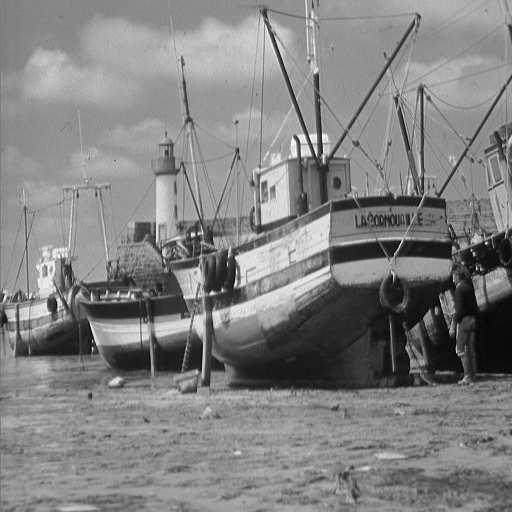
\includegraphics[width=0.35\textwidth]{figures/exams/boat.png}
            } \hfill %
            \subfloat[$ M^{\leftrightarrow} $]{
                \label{fig:hflip}
                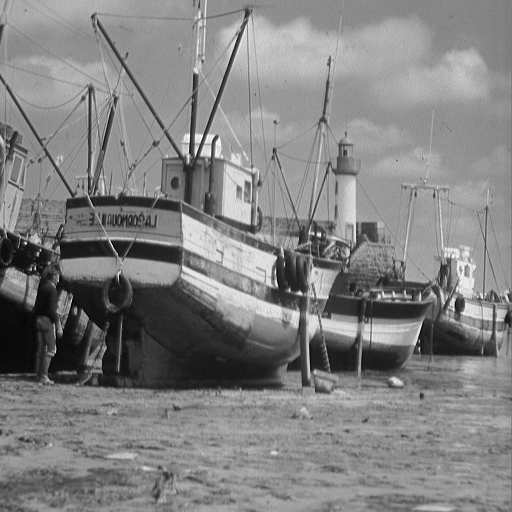
\includegraphics[width=0.35\textwidth]{figures/exams/boat_hflip.png}
            }\hfill\null \\
            \null\hfill
            \subfloat[$ M^{\updownarrow} $]{
                \label{fig:vflip}
                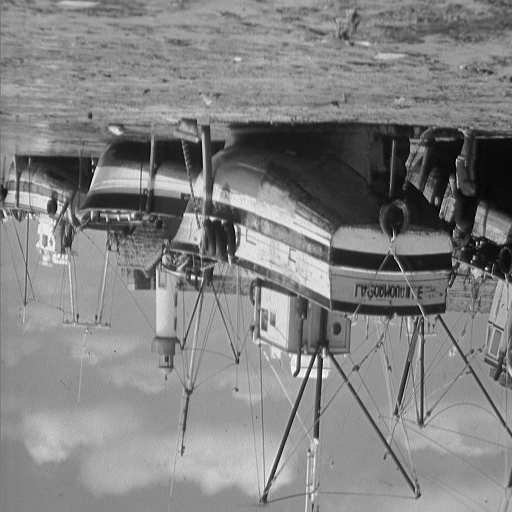
\includegraphics[width=0.35\textwidth]{figures/exams/boat_vflip.png}
            } \hfill %
            \subfloat[$ M^T $]{
                \label{fig:transpose}
                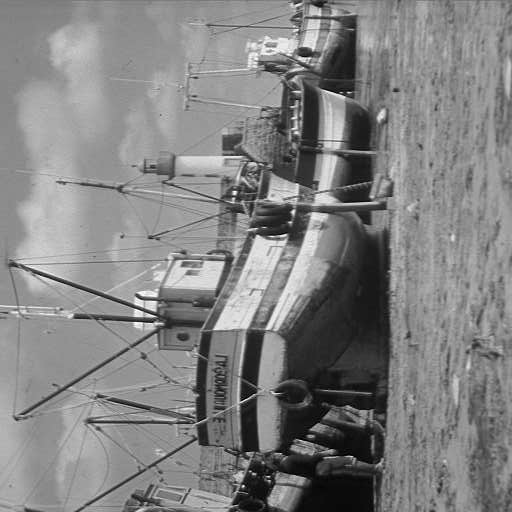
\includegraphics[width=0.35\textwidth]{figures/exams/boat_transpose.png}
            } \hfill\null
        \end{center}
        \caption{Exemple d'opérations géométriques sur une image}
        \label{fig:boat}
    \end{figure}

\correctionExam{Manipulation d'images, requêtes SQL}{18-03-2023}

\section*{Requêtes SQL}
\ques Les espaces, l'indentation, les retours à la ligne, le choix de majuscule/minuscule n'importent pas.
\ssques \mintinline{sql}{SELECT Title FROM publication;}
\ssques \begin{minted}{sql}
    SELECT Title, Year
        FROM publication
        ORDER BY Year ASC
        LIMIT 5;
\end{minted}
\ssques \begin{minted}{sql}
    SELECT Count(*)
        FROM publication
        WHERE Year > 1980;
\end{minted}

\ssques \begin{minted}{sql}
    SELECT p.Title
        FROM publication as p JOIN author as a ON a.Article = p.DOI
        WHERE a.Name = "Curie" AND a.FirstName = "Marie";
\end{minted}

\ssques \begin{minted}{sql}
    SELECT a.Name, p.Title
        FROM publication as p JOIN author as a ON a.Article = p.DOI
        WHERE a.Rank = 1 AND p.Year > 2000 AND p.Field = "Biology";
\end{minted}

\ssques \begin{minted}{sql}
    SELECT a1.Name
        FROM author as a1 JOIN author as a2 ON a1.DOI = a2.DOI
        WHERE (a1.Name != "Turing" OR a1.FirstName != "Alan")
            AND a2.Name = "Turing" AND a2.FirstName = "Alan";
\end{minted}

\section*{Manipulation d'images}

\ques
\ssques $ M^{\leftrightarrow} $ a la même dimension que $ M $, donc $ m \times n $
\ssques $ M^{\leftrightarrow}_{i,j} = M_{i, n-j} $
\ssques \begin{minted}{python}
    def  reflexion_horizontale(img):
        h, w = np.shape(img)
        ret = np.zeros((h, w))
        for i in range(h):
            for j in range(w):
                ret[i, j] = img[i, w-1-j]
        return ret

    # ou encore
    def  reflexion_horizontale(img):
        return img[:, ::-1]
\end{minted}

\ques
\ssques $ M^T $ a dimension $ n \times m $.
\ssques $ M^t_{i,j} = M_{j, i} $
\ssques \begin{minted}{python}
    def transpose(img):
        h, w = np.shape(img)
        ret = np.zeros((w, h))
        for i in range(w):
            for j in range(h):
                ret[i, j] = img[j, i]
    return ret

    # ou encore
    def transpose(img):
        return img.T
\end{minted}

\ques
\ssques $ M^{\updownarrow} $ a la même dimension que $ M $, donc $ m \times n $
\ssques $ M^{\updownarrow}_{i, j} = M_{m-i, j} $
\ssques On montre l'égalité coefficient par coefficient :
\begin{align*}
    (M^T)^{\leftrightarrow}_{i,j} &= M^T_{i, m-j} \quad \textrm{car $ M^T $ est de dimension $ n \times m $} \\
                                  &= M_{m-j, i} \\
    (M^{\updownarrow})^T_{i,j} &=  M^{\updownarrow}_{j,i} \\
                               &= M_{m-j, i}
\end{align*}
\ssques Il suffit de prendre la transposée de l'égalité prouvée à la question précédente.

\ques 

\begin{minted}{python}
    def reflexion_verticale(img):
        return transpose(reflexion_horizontale(transpose(img)))

    # pas la solution attendue, mais on peut aussi écrire
    def reflexion_verticale(img):
        return img[::-1, :]
\end{minted}



\end{document}
